%-----------------------------------------------------------------------------------------------------------------
\chapter{Related Work}
\label{cap2:related_work}

%-------------------------------------------------------------------------------------------------------------
Given the vast range of research works in the robotic grasping, this chapter discusses and reviews state-of-the-art proposals of grasping solutions and how they evolved over the years. This chapter build the basis to the thesis proposals.

%It also discusses and presents the new steps and future works ideas not yet explored: from the academic field to the new challenges of industry 4.0. 

%Moreover, the first Ph.D contribution is presented. It formalises and standardises the grasping evaluation idea since a grasping problem involves perception, planning, and control. Therefore, a clear standard could improve the methodologies' comparability since each step of the procedure affects the grasping performance. 

The remainder of the chapter is organised as follows: Section~\ref{cap2:related_work:sec:grasping_representation} shows and discusses the different grasping representations since the characterisation is the most important step to any grasping planning approach. A review of Analytical, Learning and Deep Learning methods is given in Sections~\ref{cap2:related_work:sec:grasping_approaches:subsec:analytical_review}, \ref{cap2:related_work:sec:grasping_approaches:subsec:learning_review}, and \ref{cap2:related_work:sec:grasping_approaches:subsec:deep_learning_review}, respectively.

%Section~\ref{sec:grasping_evaluation} presents a grasping evaluation discussion following by our proposal.  The discussion, exploration of future works ideas, and the conclusion are presented in Sections~\ref{sec:discussion_and_future_work}, and ~\ref{sec:conclusion}, respectively. 


%The rest of the paper is divided as follow: after the introduction section, a grasping definition %problem is introduced in Section~\ref{sec:grasping_definition_problem}, formalizing the discussion %along the paper. Section~\ref{sec:grasping_representation} shows and discuss the types of grasping %representation. A review about Analytical, Learning and Deep Learning methods are given in %Sections~\ref{sec:analytical_review}, \ref{sec:learning_review} and \ref{sec:deep_learning_review}, %respectively. The Section~\ref{sec:grasping_evaluation} presents a grasping evaluation discussion %following by our proposal.  In the end, the conclusion is presented in Section~\ref{sec:conclusion} %exploring future works ideas. 


% \section{The Robotic Grasping Problem}\label{sec:grasping_definition_problem}

% The robotic grasping affordance is related to perform a set of contacts (or stay near, in the case of magnetic and suction gripper) between the active pairs (the workpiece and the gripper). Typically, as related by~\cite{Ghazaei2019}, a grasping procedure can be divided in three parts: perception, planning and control. An detailed example description of this common proposal is presented in the Figure~\ref{fig:grasping}. 


%\begin{figure}[h]
%    \centering
%    \includegraphics[scale=0.5]{example-image-a} 
%    \caption{XXX}
%    \label{fig:grasping}
%\end{figure}{}



\section{Grasping Representation}
\label{cap2:related_work:sec:grasping_representation}


There are several approaches regarding how to represent a grasping, i.e., how to describe and characterise it. This subject is a valuable step to the development of grasping planning or grasping detection algorithms and will be discussed in this section.  


Some approaches model the physical interaction between the active pairs and evaluate its equilibrium and stability performance with the wrench space analyses and Coulomb's law in multi-fingered grasping (Figure~\ref{fig:friction_contact}). It is a prevalent approach in analytical methodologies~\cite{liu2004complete,el2009computing, miller2004graspit, AndrewT2004} and present in Learning and \ac{DL} policies~\cite{Mahler2016, Mahler2017b, Mahler2017d, Mahler2017, Mahler2019}. Typically, it depends on the active pair's 3D shape (Point-Cloud, Voxel Grids, or 3D models) since the contacts need to be evaluated in an iteration algorithm or simulation. Well-recognised quality metrics are the Convex Hull's volume and the Epsilon radius of the grasping wrench space configuration proposed by \citeauthor{Ferrari} in~\cite{Ferrari} (Figure~\ref{fig:gws_force_closure_main}). Since a complete wrench space analyses  demand effort, a simplified modelling strategy is the antipodal restraints~\cite{Nguyen1987_1} represented by Figure~\ref{fig:antipodal}, which is commonly used by proposals that employ two-finger grasping. 

\begin{figure}[h!] %because of cas-sc
\resizebox{.7\textwidth}{!}{%
\begin{tcolorbox}
\centerline{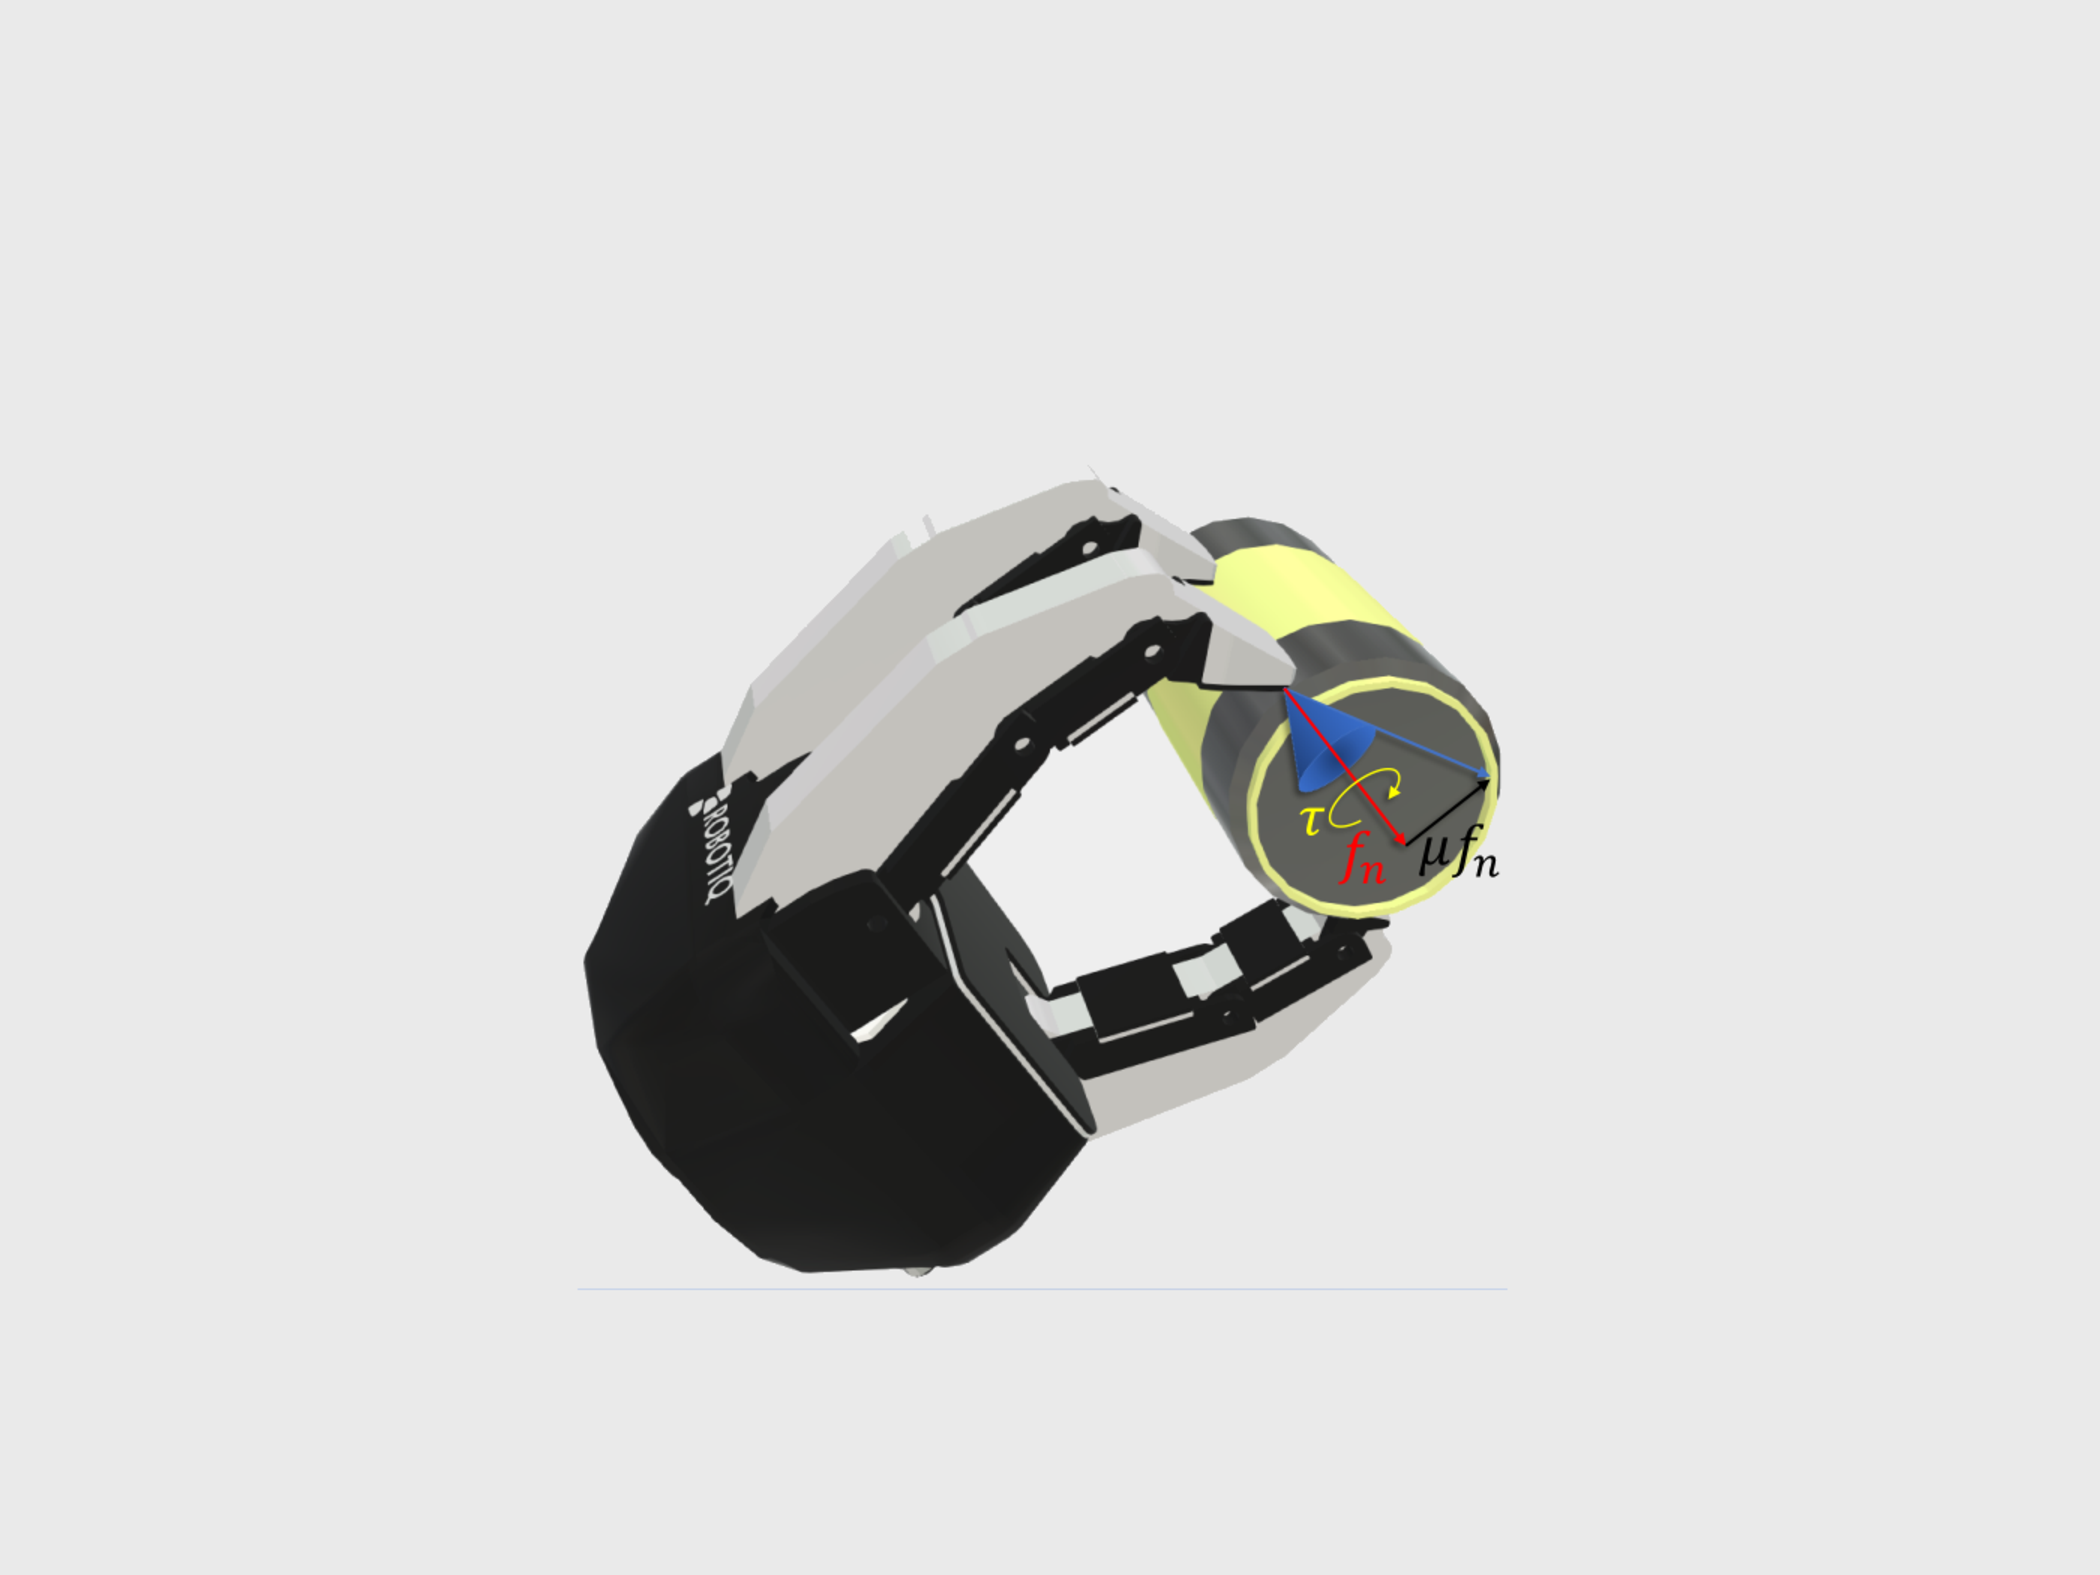
\includegraphics[trim={10cm 5cm 10.2cm 8cm},clip,width=.75\linewidth,angle=0]{Cap2/Figuras/grasp.pdf}}
\end{tcolorbox}
\caption{Soft finger friction contact model.}
\label{fig:friction_contact}
\label{fig:}
}
\end{figure}



% \begin{figure}[h]
%     \centering
%     \includegraphics[scale=0.5]{example-image-a} 
%     \caption{Wrench space analyses and Coulomb’s law}
%     \label{fig:wrench_space_coulombs_theory}
% \end{figure}

% \begin{figure}[h]
%     \centering
%     \includegraphics[scale=0.5]{example-image-a} 
%     \caption{Convex Hull's Epsilon and Volume grasping representation: normally the task is to find the finger's poses over the object and evaluate the epsilon and volume values.}
%     \label{fig:epsilon_and_volume}
% \end{figure}


% \begin{figure}[h!] %because of cas-sc
% % \centerline{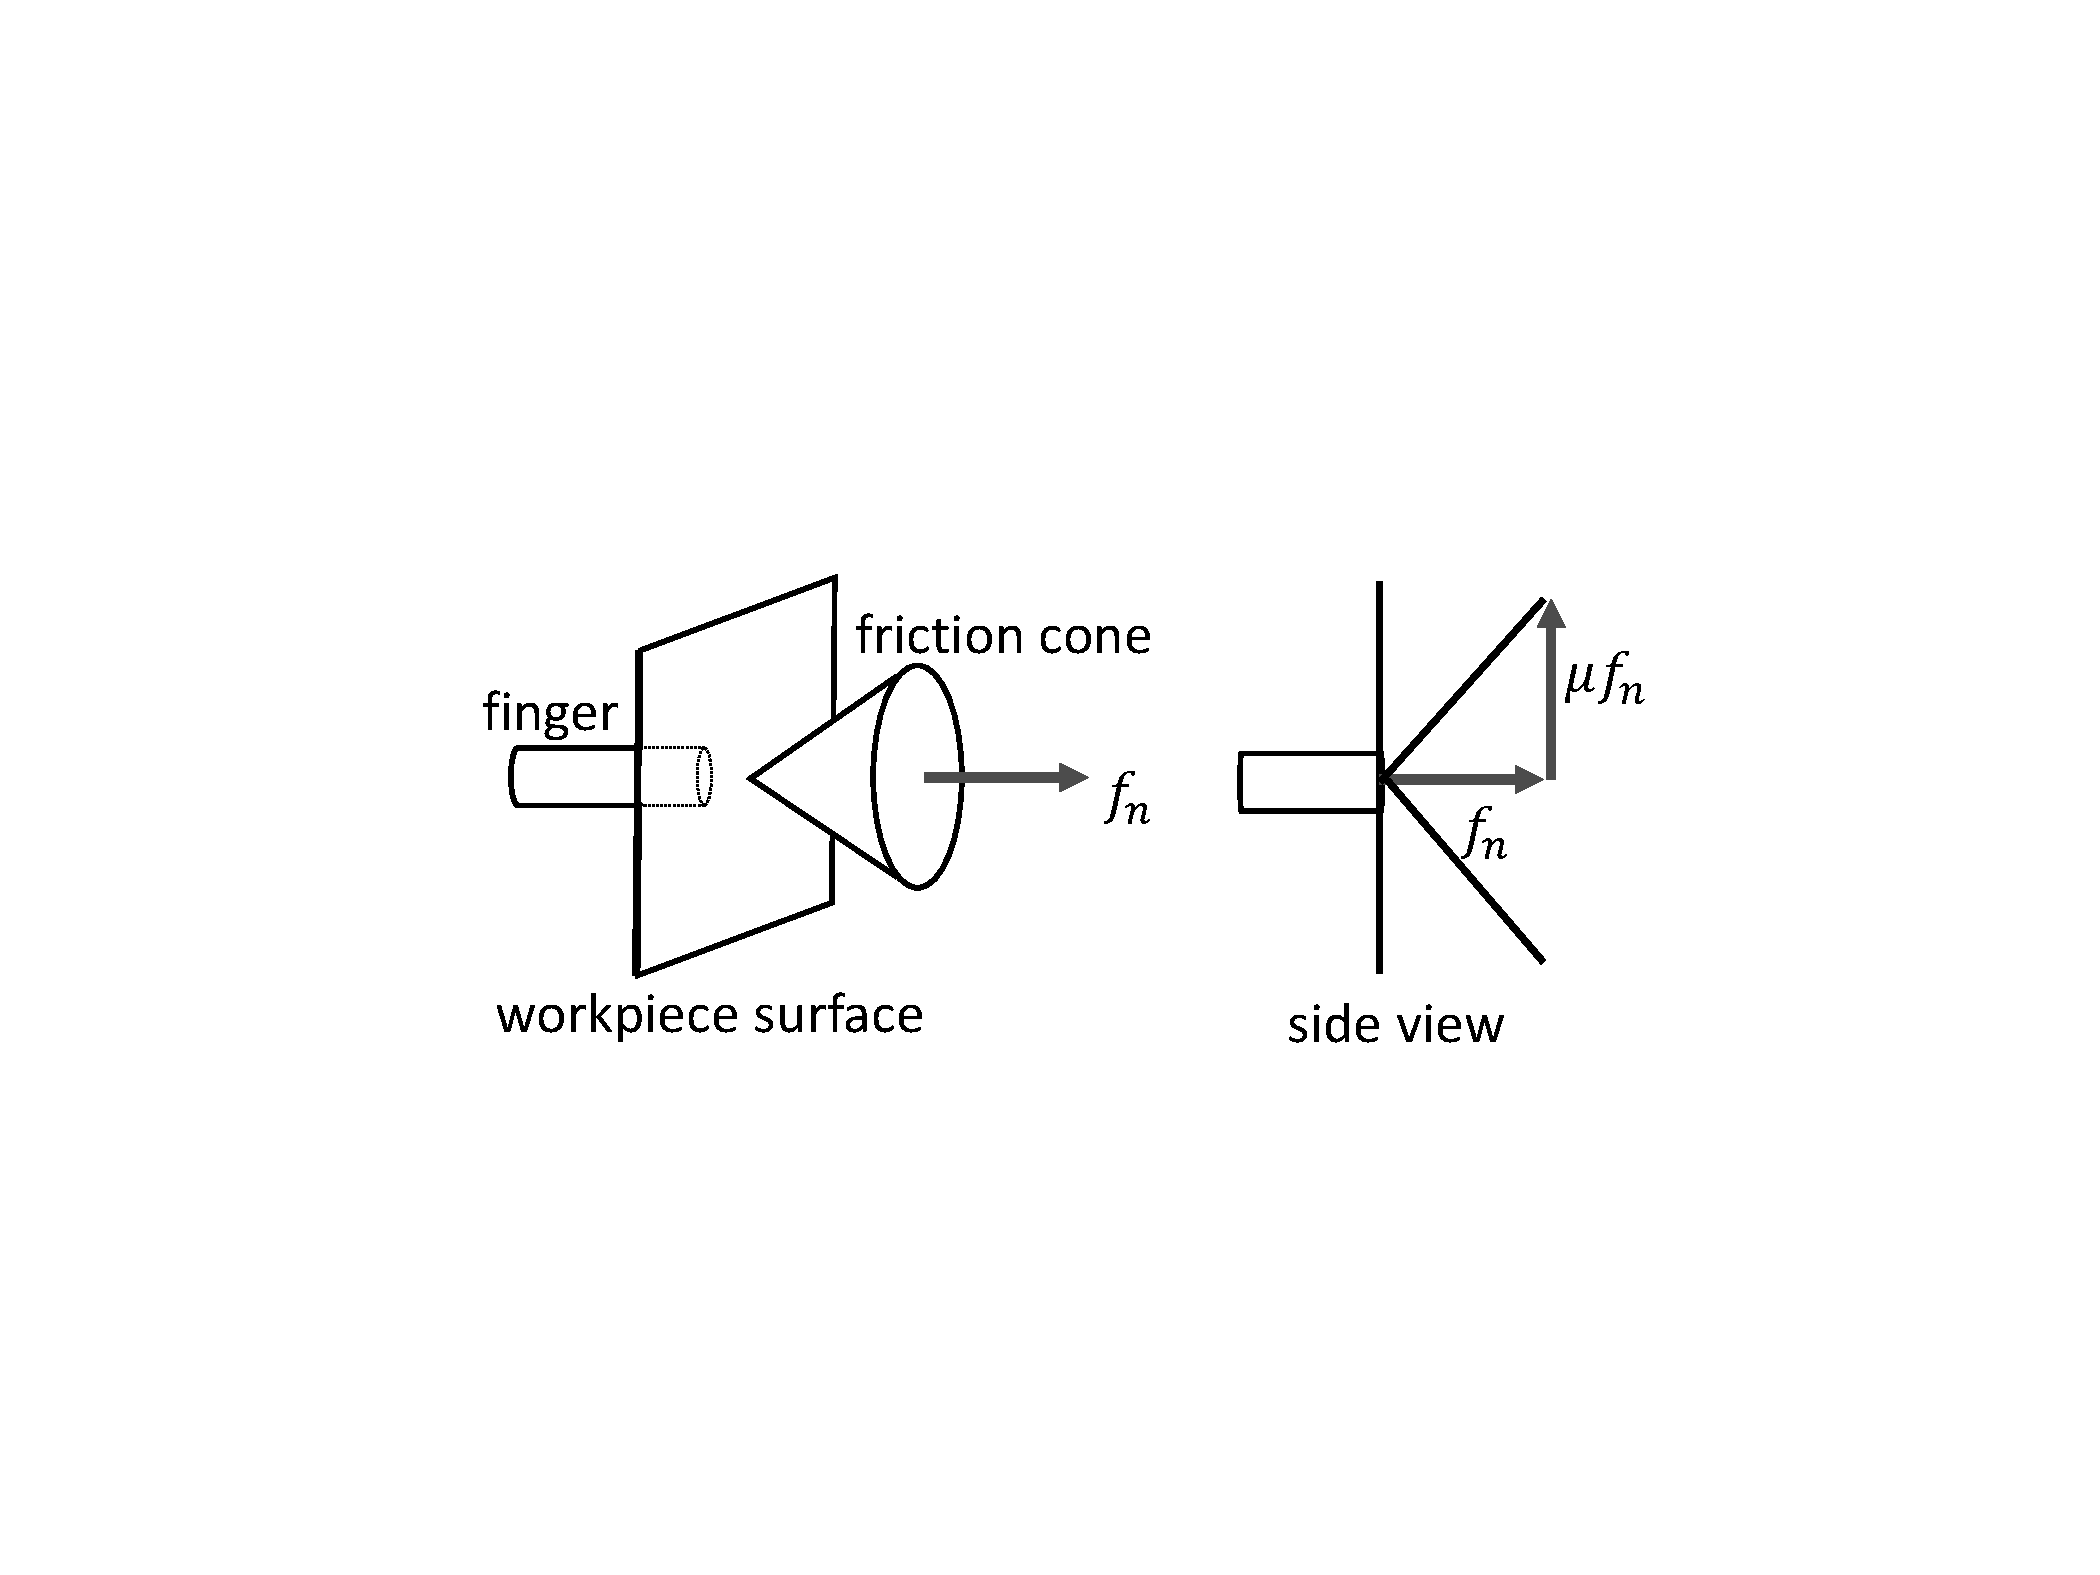
\includegraphics[trim={7cm 8cm 7cm 9cm},clip,width=1\linewidth,angle=0]{Cap2/Figuras/friction_contact.pdf}}
% \centerline{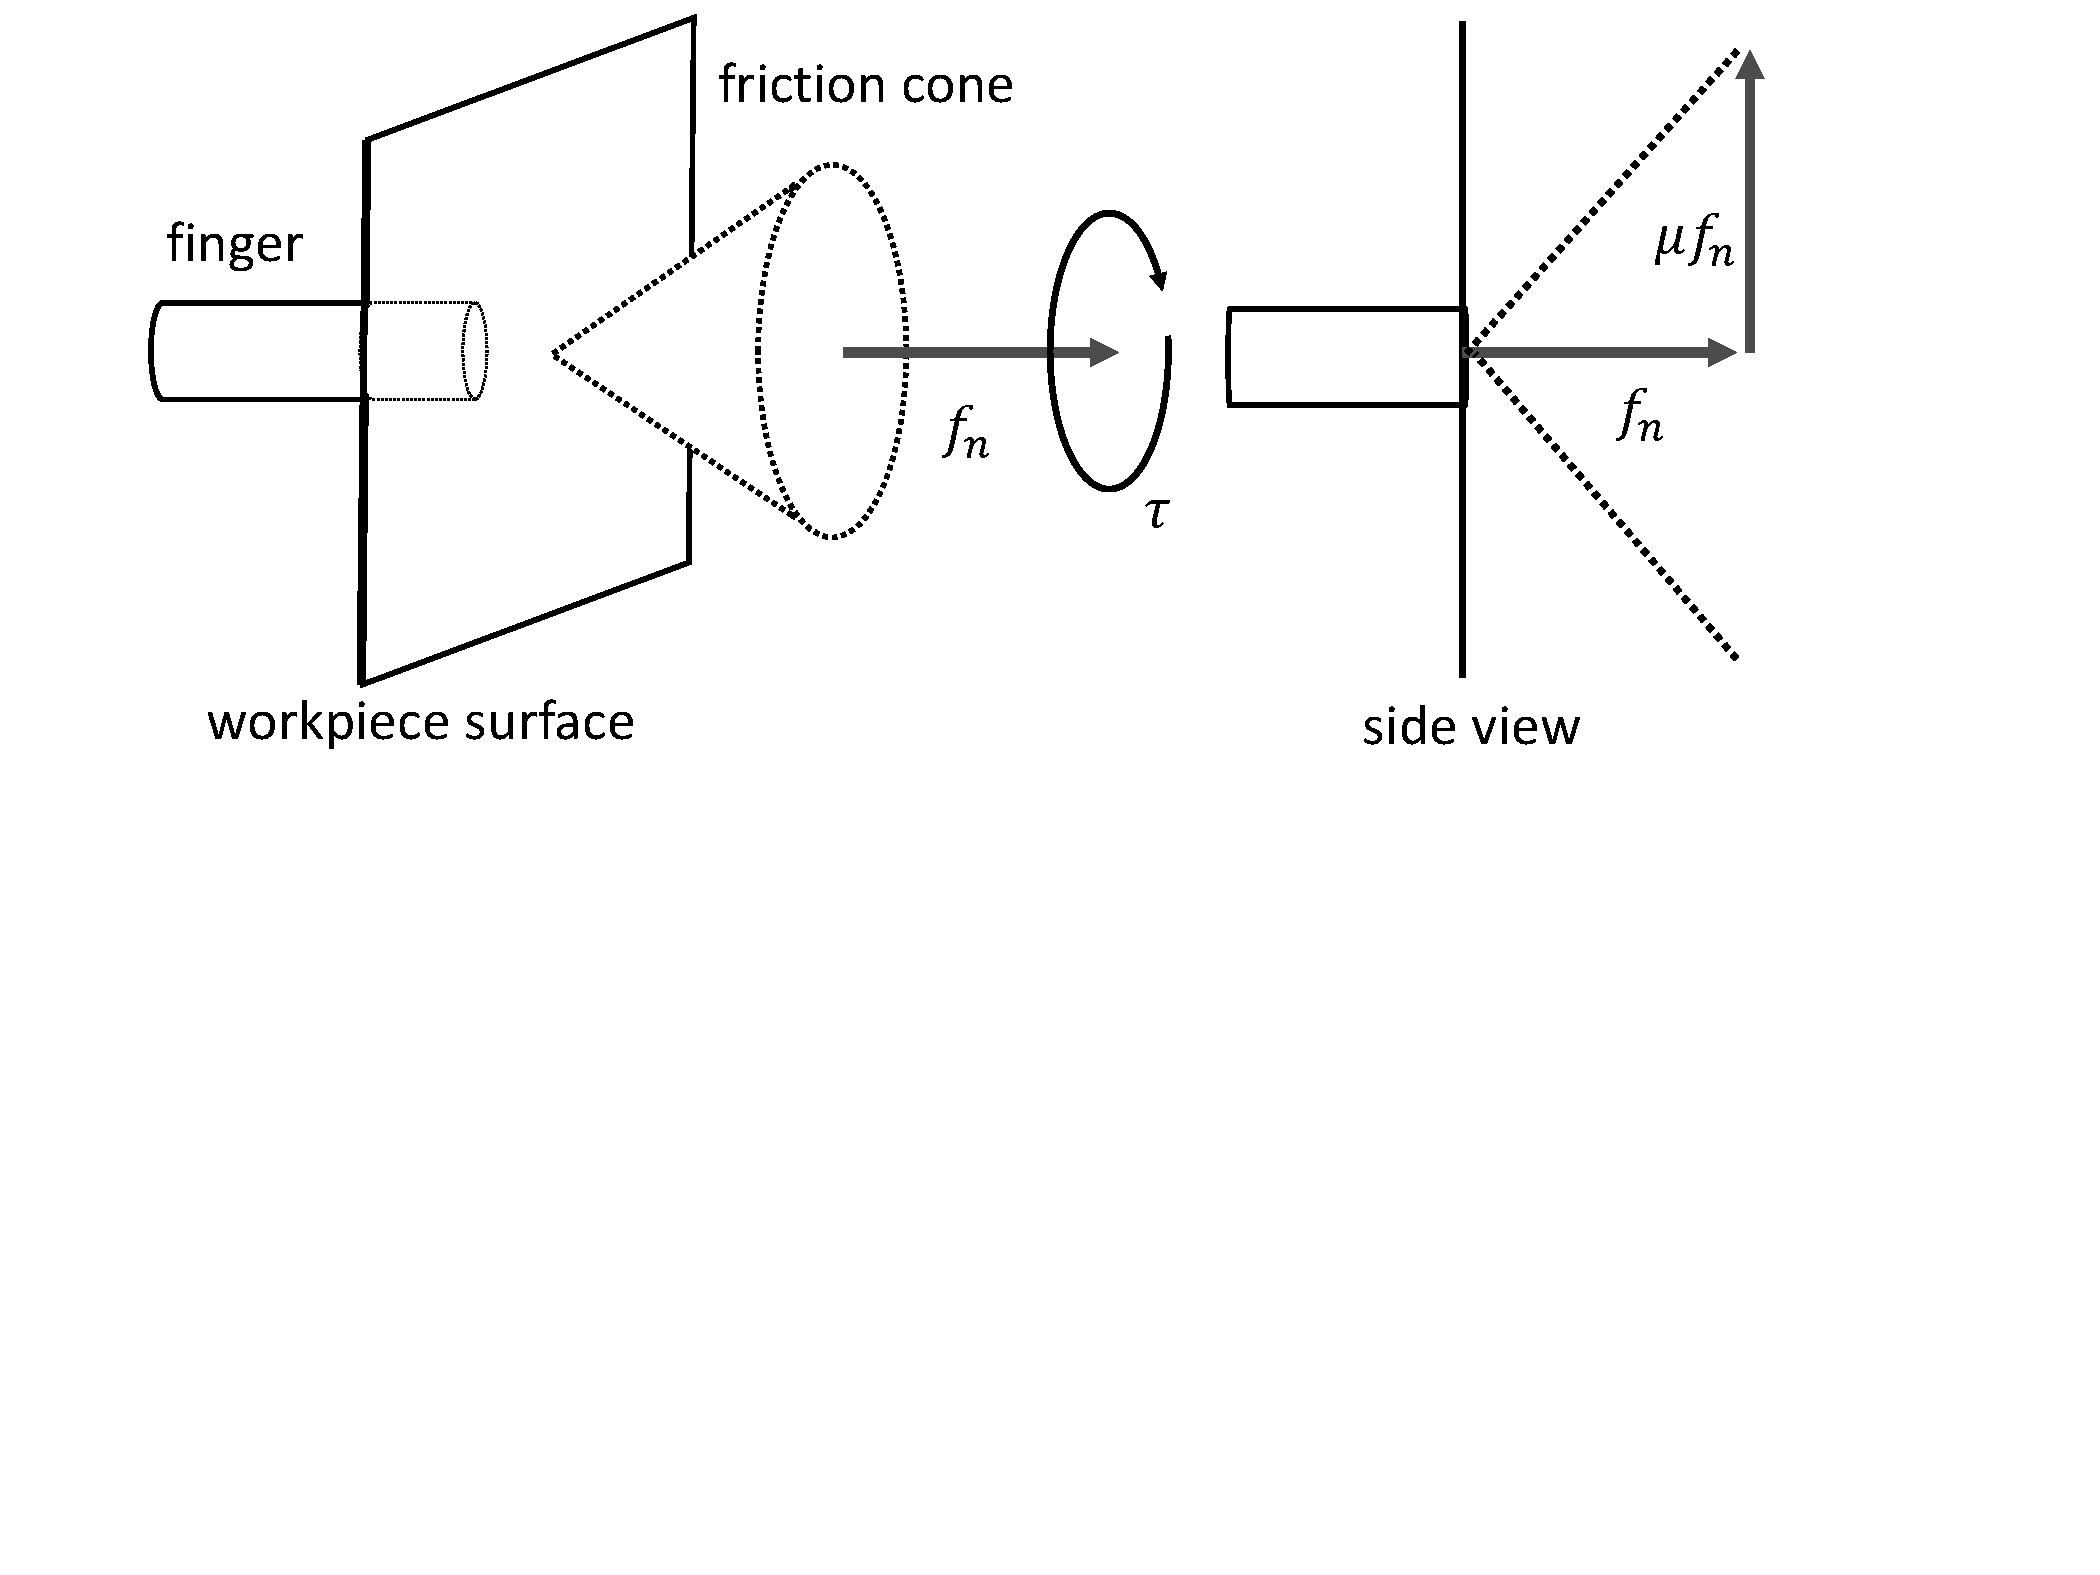
\includegraphics[trim={2.5cm 14cm 5.7cm 0cm},clip,width=.85\linewidth,angle=0]{Cap2/Figuras/soft_finger_contact.pdf}}
% \caption{A soft friction contact model and the geometric representation of Coulomb’s law (figure based on~\cite{murray1994mathematical}). }
% \label{fig:friction_contact}
% \end{figure}


In many applications,  the model shapes unfamiliarity is a significant drawback, and the ability to exceed the grasping to novel objects is necessary. This capability is also referred to as object-agnostic grasping. Decomposition heuristics and learning algorithms try to solve this issue. Even though, in most cases, the gripper topology generalisation is not considered. The point~\cite{Saxena2008} and the oriented rectangle grasping representations~\cite{Jiang2011a} (Figure~\ref{fig:exemples_rep}) were the options of several works to find a grasping pose over an object. These metrics, used in \ac{SL} methodologies, commonly require a labelled ground-truth, as \ac{CGD}~\cite{conerll_database} and Jacquard~\cite{jacquard_dataset} datasets. The point representation, normally indicated by a 3D pose, has a lack of physical limitation descriptors, like gripper's width and orientation approach angle, which are included in the rectangle methodology, see Figure~\ref{fig:exemples_rep}. The point representation metric only evaluates a distance between the detected grasping pose and the ground-truth, while the rectangle is also evaluated by the Jacquard threshold (Figure~\ref{fig:pen_jacquard}).


\begin{tcolorbox}[every float=\centering, drop shadow, title= Wrench Space Analyses]
Each contact can be modelled by a wrench vector $\mathbf{w}$ composed of forces and torques. All contact wrenches associated mould the convex-hull configuration, which can evaluate a grasping equilibrium. In a case of planar multi-fingered grasp, a force-closure grasp has the wrench space origin included by its convex-hull geometry (left convex-hull of Figure~\ref{fig:gws_force_closure_main}), unlike a non-force closure (right convex-hull of Figure~\ref{fig:gws_force_closure_main}). The $\epsilon$ is an example of the quality value to define the best force-closure configuration. It represents the wrench vector's distance to the origin ($\{O\}$), which is the shortest, i.e., the worst wrench vector to support an external perturbation.

\vspace*{1ex}

% \centerline{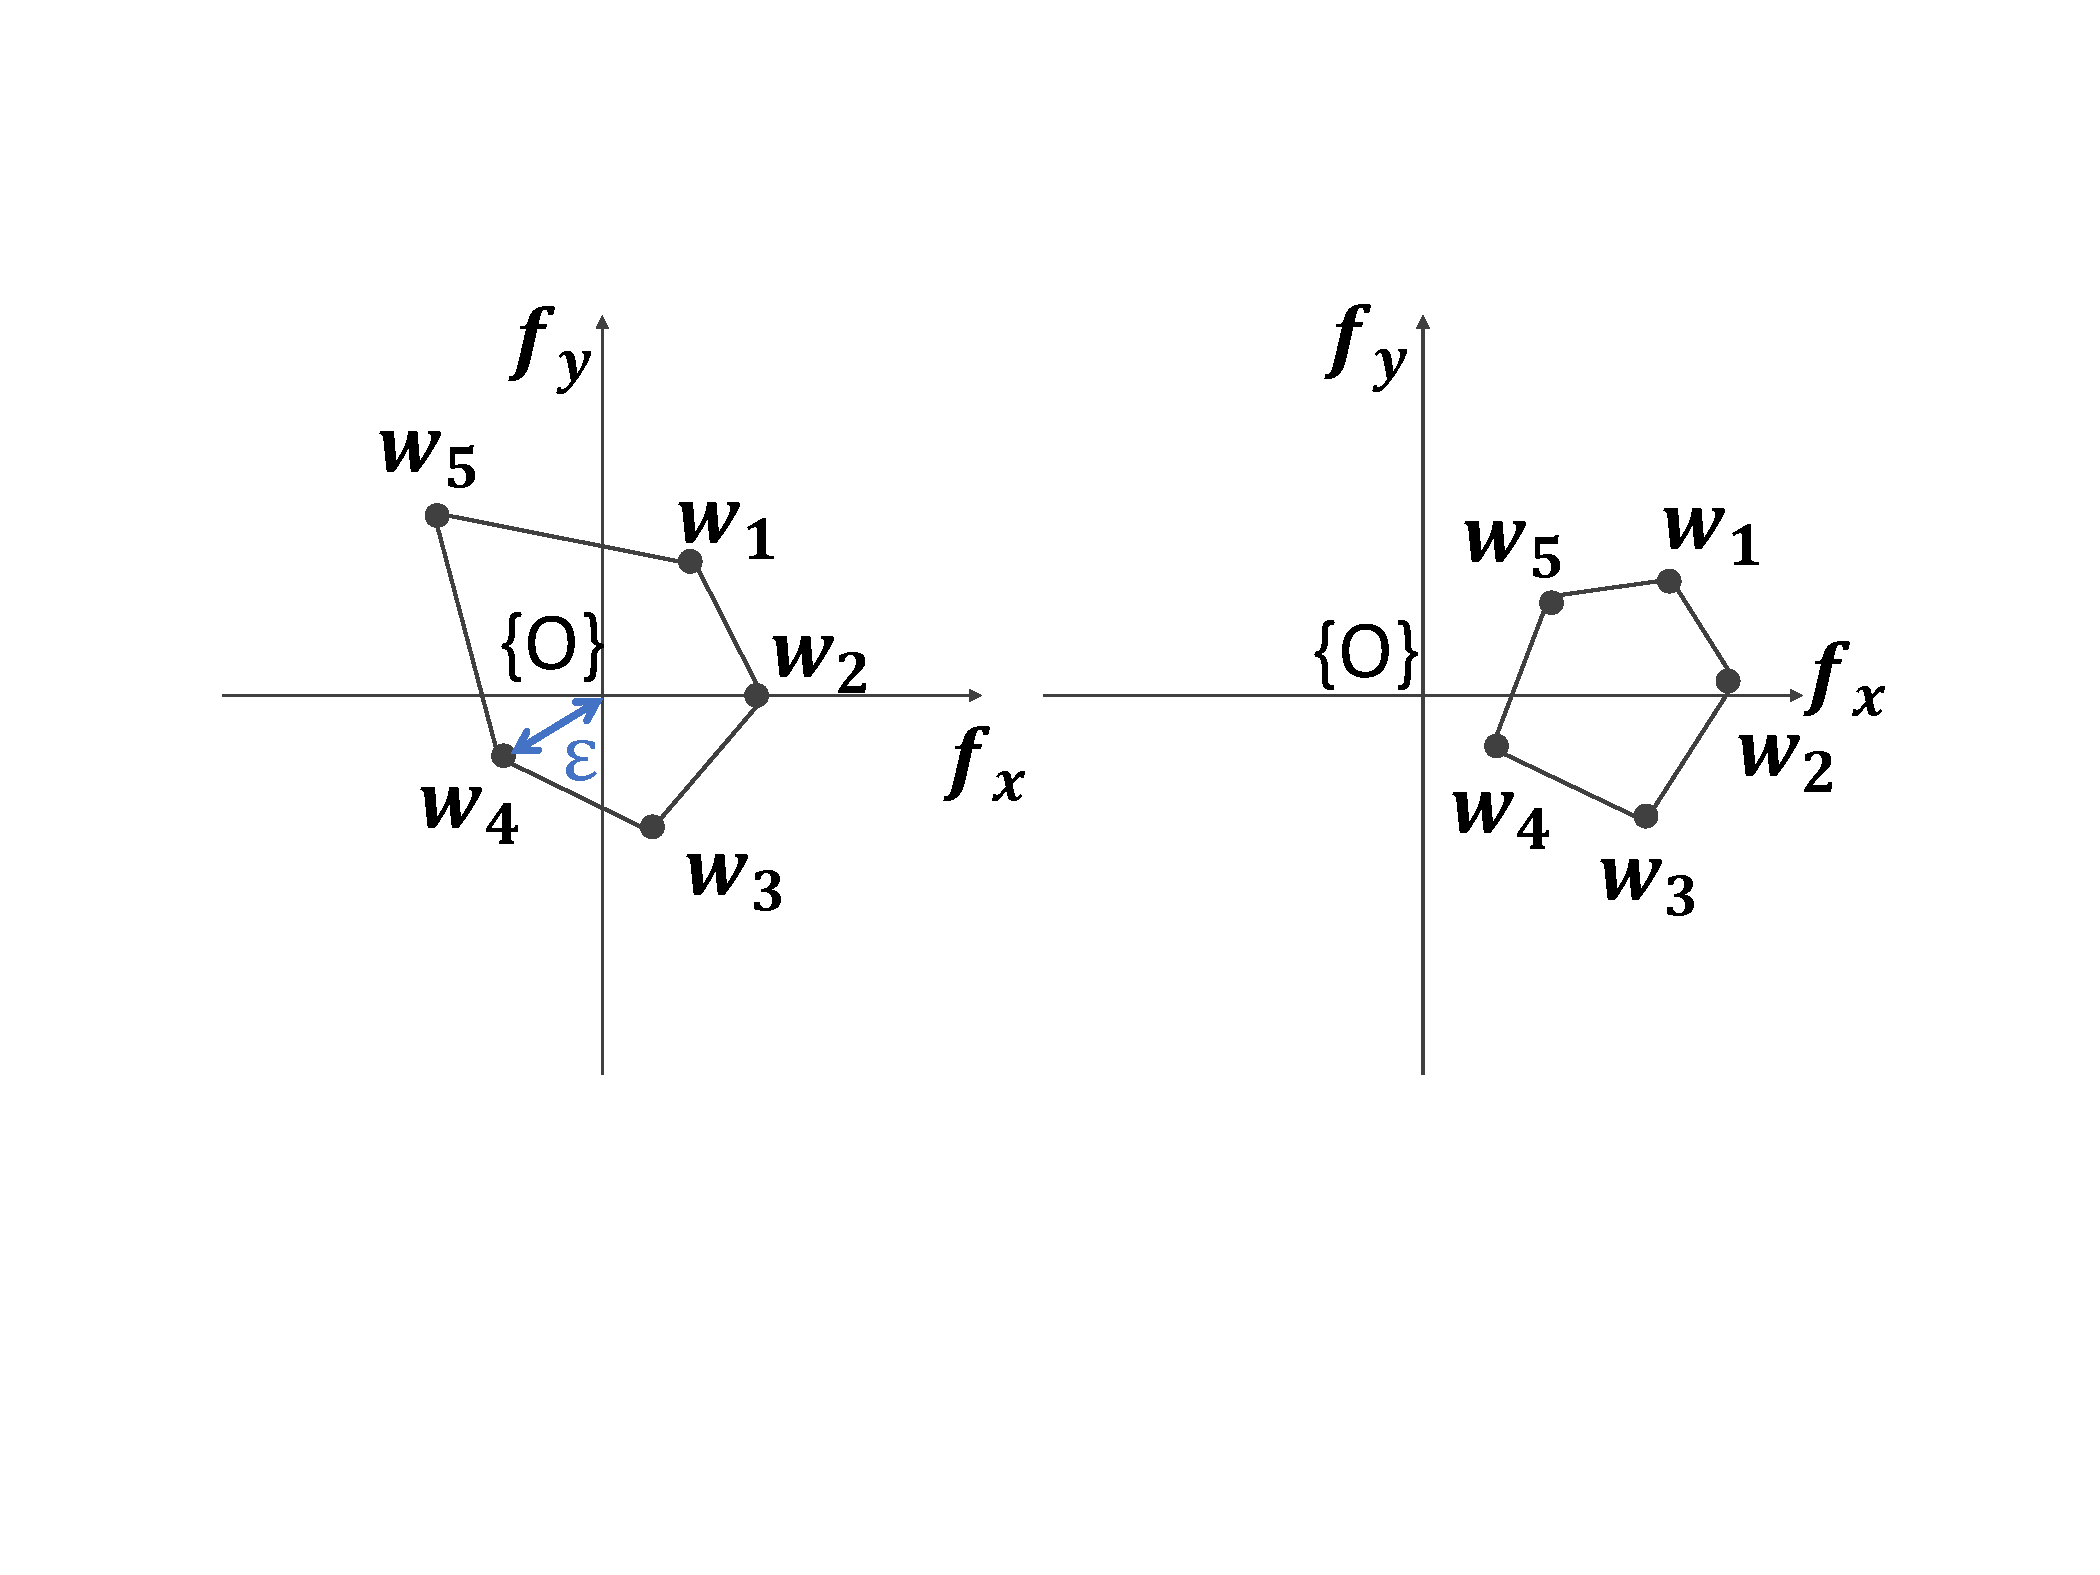
\includegraphics[trim={4cm 10cm 3cm 5cm},clip,width=1\linewidth,angle=0]{Cap2/Figuras/convex_hull_force_grasp.pdf}}
\centerline{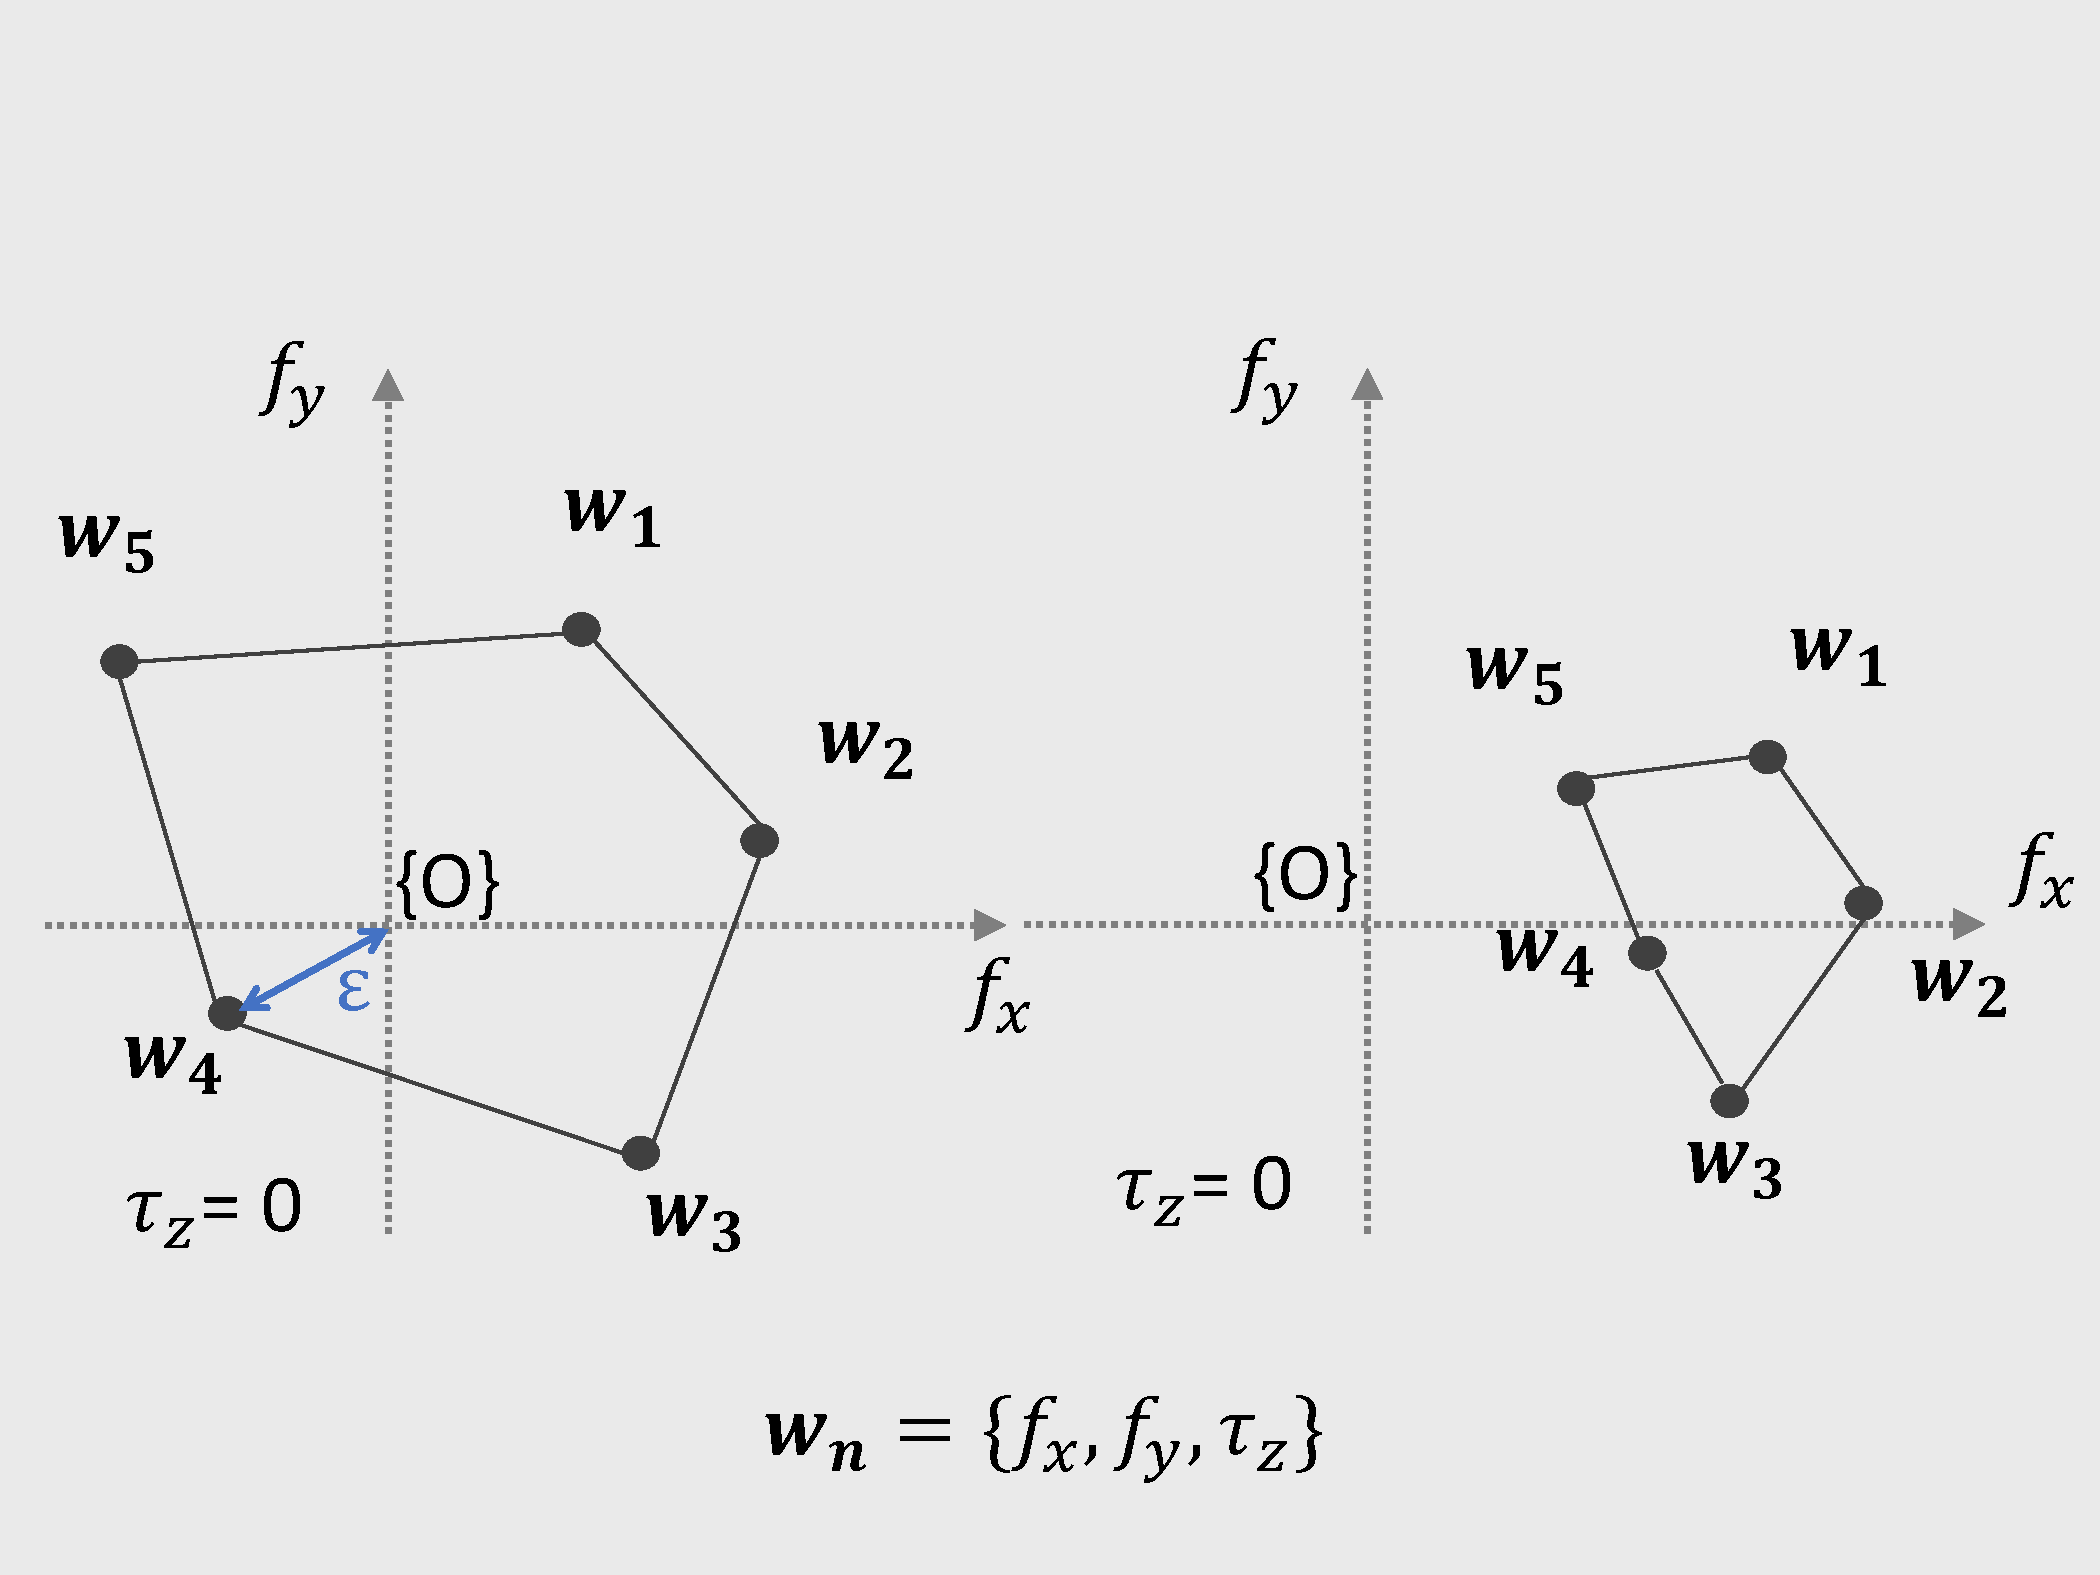
\includegraphics[trim={0cm 1.2cm 0cm 5.5cm},clip,width=0.65\linewidth,angle=0]{Cap2/Figuras/wrenchspace_anlayses_2.pdf}}
\captionof{figure}{Wrench space analyses representation}\label{fig:gws_force_closure_main}
\end{tcolorbox}

Following~\cite{Jiang2011a}, \citeauthor{Lenz2015}~\cite{Lenz2015} propose that the 6DOF-Rectangle could be simplified and confirm that this representation can be projected back to a 3DOF space. However, the authors do not explain this mapping. Later works~\cite{Redmon2015,Watson2017,Gariepy2019,asif2018ensemblenet} used this approach and achieved an interesting grasping detection success rate. 

\begin{tcolorbox}[every float=\centering, drop shadow, title= Antipodal Grasping]

 Two-finger contact with friction can be defined as force-closure if, and only if,  the line that connects each contact lays inside both friction cones. A non-force closure and a force closure antipodal grasping are represented by the left and right grasps of Figure~\ref{fig:antipodal}, respectively.

\vspace*{1ex}

\centerline{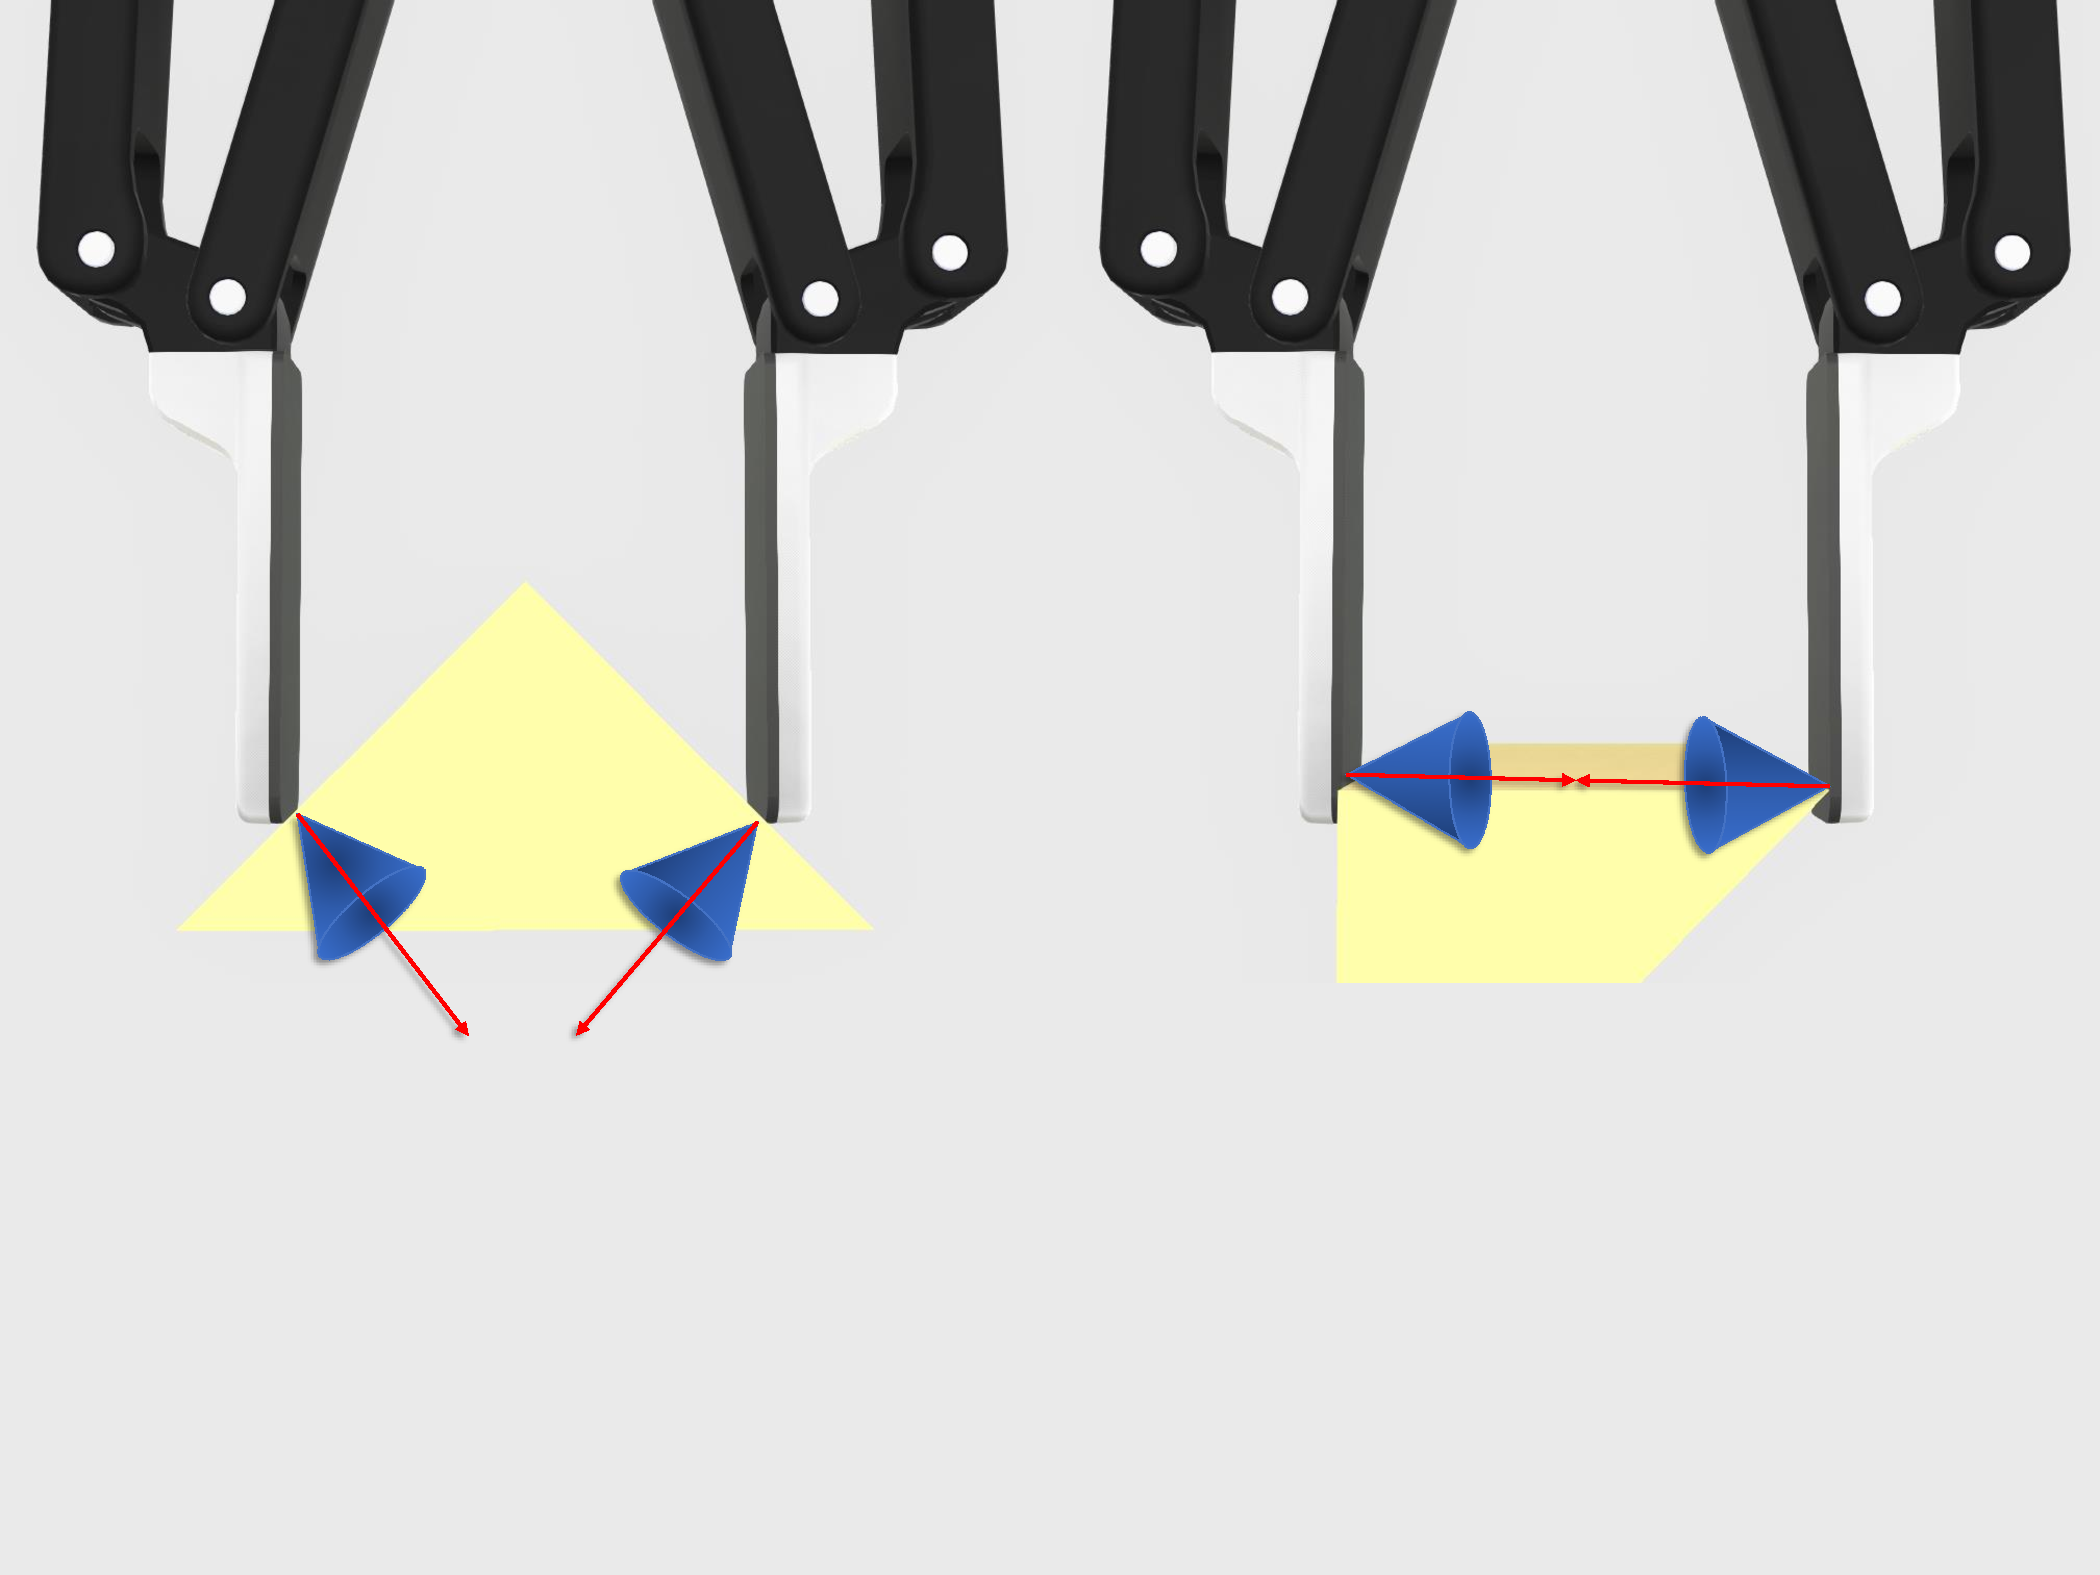
\includegraphics[trim={0cm 10cm 0cm 0cm},clip,width=.5\linewidth,angle=0]{Cap2/Figuras/antipodal_2.pdf}}
\captionof{figure}{Antipodal grasping restriction}\label{fig:antipodal}
\end{tcolorbox}


Even if several state-of-the-art works use these image-based metrics to assess the efficiency of grasping detection, this approach is questionable ~\cite{Guo2017,Gariepy2019,Mousavian_2019_ICCV,Ghazaei2019,TenPas2017,choi2018learning, Chen2019}. Some authors~\cite{Gariepy2019,Ghazaei2019} affirm that the grasping is not completely defined like an object's classification in an image, i.e., there still exist many grasping possibilities which are not mapped in a ground-truth database. Despite the gripper's physical limitations of rectangle representation modelling,  it is possible to note that the grasping performance does not reflect several works' success detection rates. This approach does not consider the real physical interactions between active pairs, e.g., force-closure properties and Coulomb's law. It also does not consider sensing noises and robot action's inconsistencies. Thus, \citeauthor{Guo2017}~\cite{Guo2017} propose a hybrid deep learning architecture combining the visual rectangle representation and tactile sensing for robotic grasping detection. Their experiments indicate that tactile data improve the grasping detection task. \citeauthor{Ghazaei2019}~\cite{Ghazaei2019} present the grasping belief maps to generate a set of grasping over an image without classifying the object whilst considering uncertainties (Figure~\ref{fig:exemples_rep}). A similar approach of pixel-wise representation is also verified by~\cite{Zeng2018}. Another continuous approach is the Grasp Path proposed by~\cite{Chen2019,Chen2020} (see Figure~\ref{fig:exemples_rep}). Asserting that the predicted comparison with the ground-truth database could eliminate other graspable candidates that are not included in the overlap threshold, the authors of~\cite{Chen2019,Chen2020} formulated a path that leads to the set configuration of rectangular grasping poses. In their tests, Grasp Path show to be less dependent on the Jacquard threshold. 


\begin{figure}[h!]
	\resizebox{.75\textwidth}{!}{%
		\begin{tcolorbox}
			\centering
			\begin{subfigure}[c]{0.45\textwidth}
				\centering
				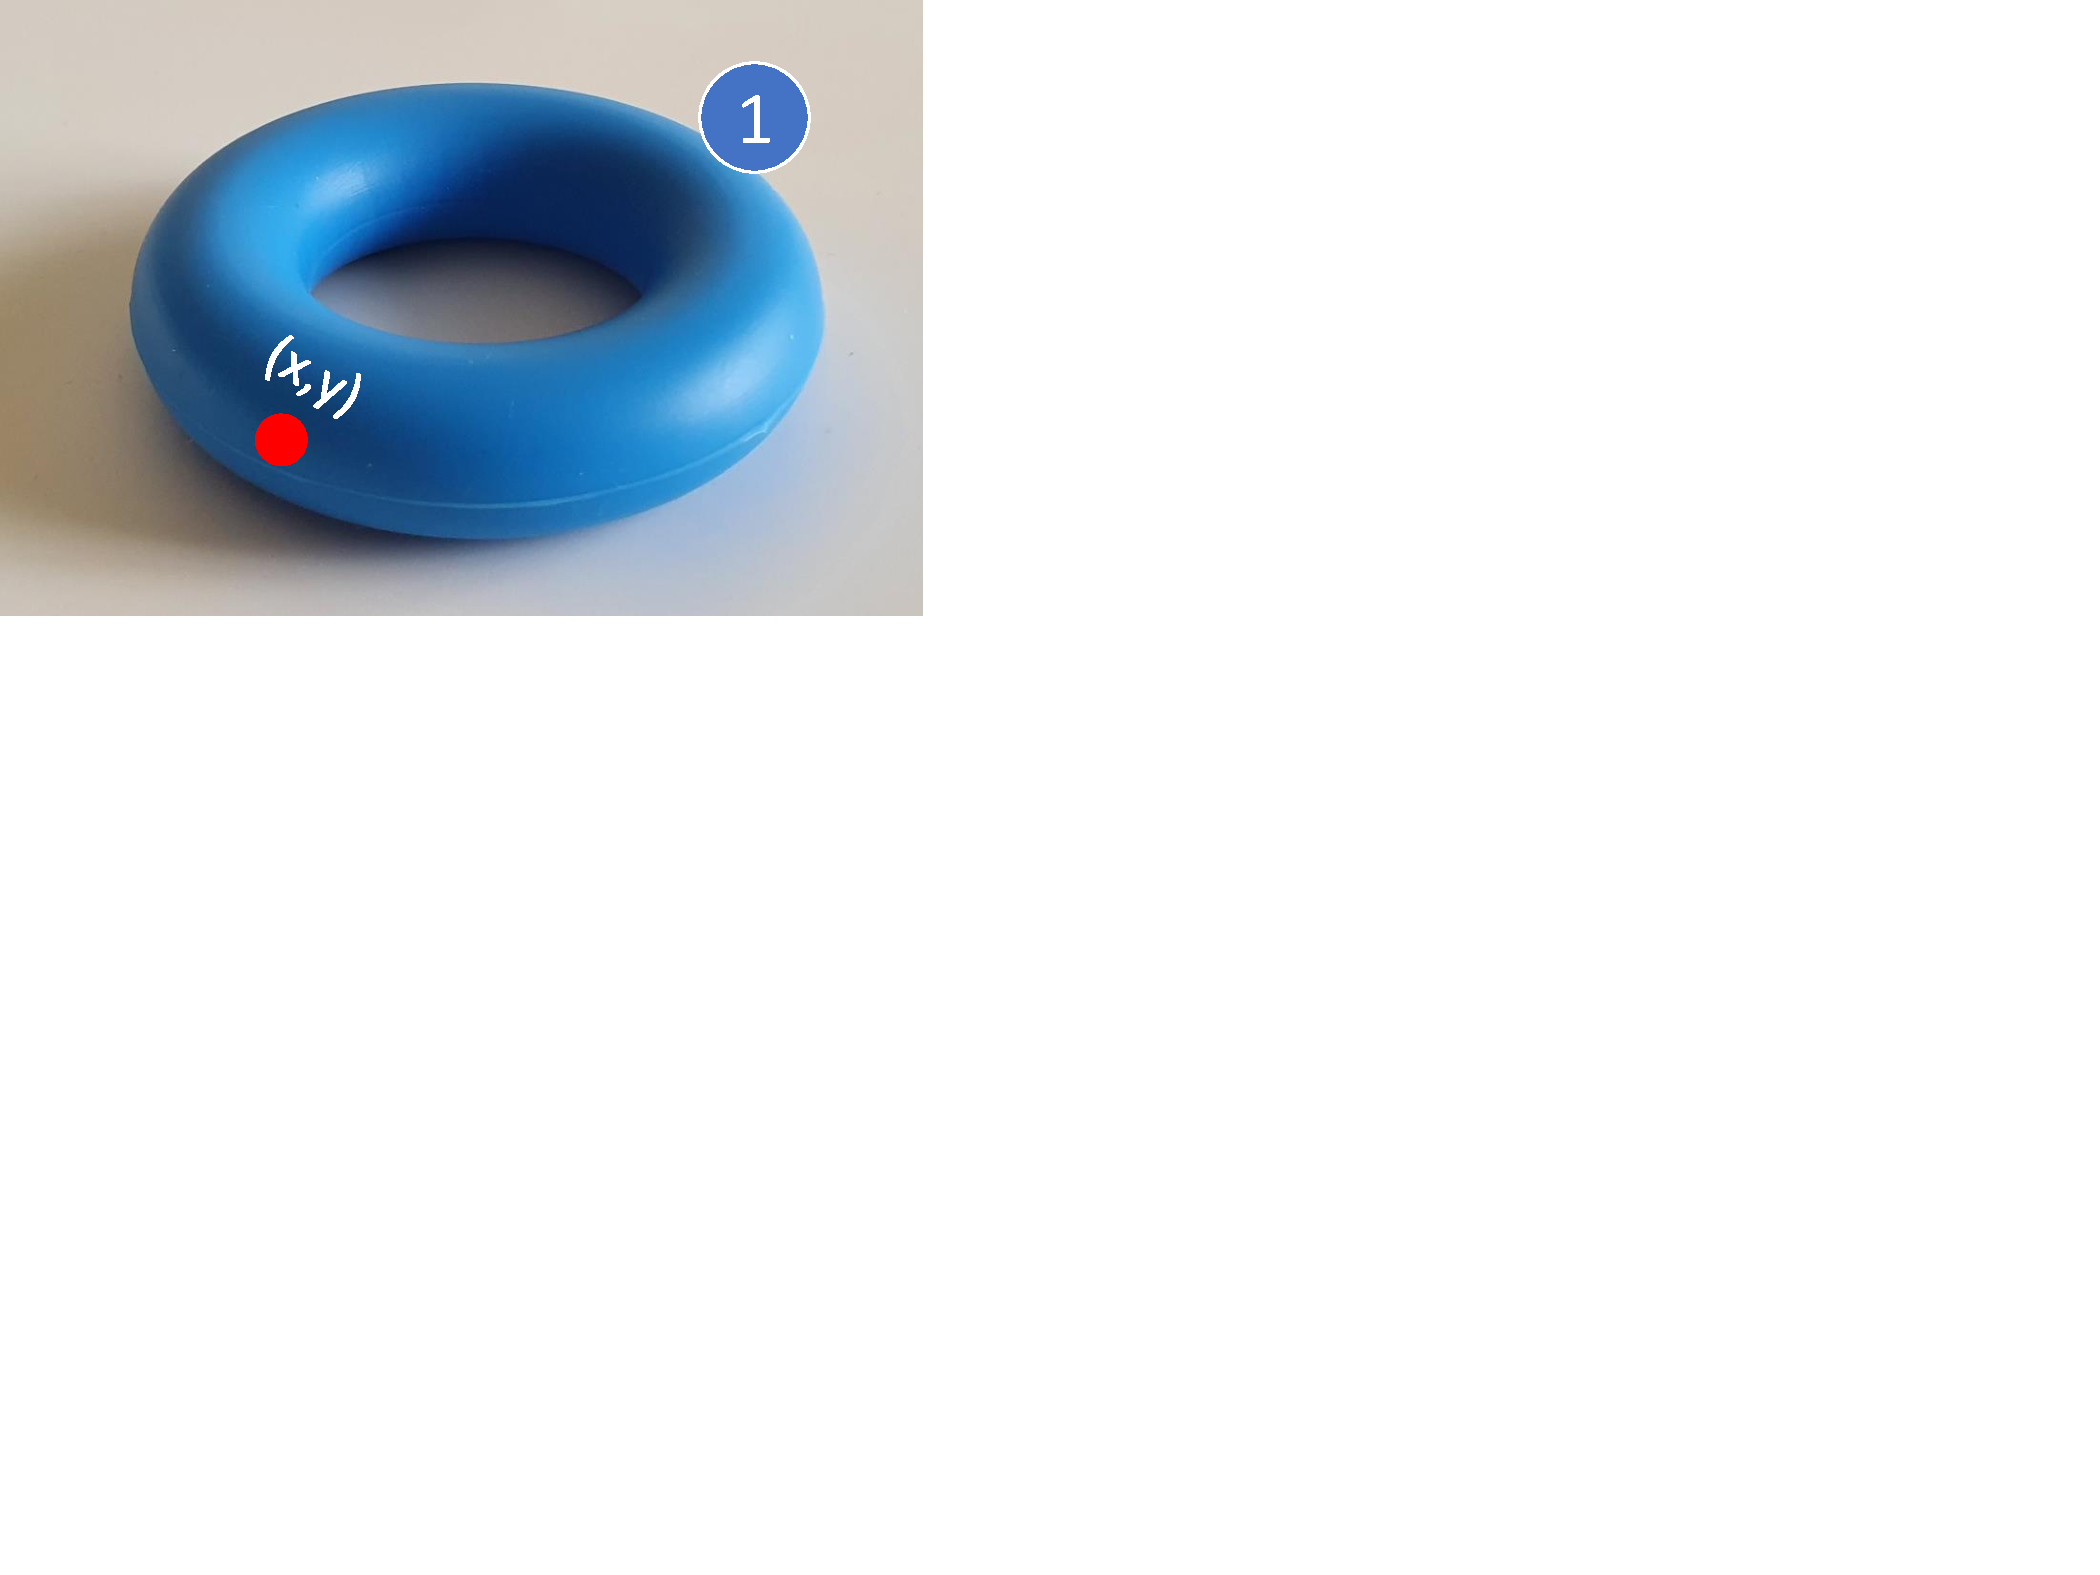
\includegraphics[trim={19mm 162mm 215mm 8mm},clip,width=1\columnwidth,angle=0]{Cap2/Figuras/point_rep.pdf}
				%\caption{Pure enclosing without clamping.}
				%\label{fig:g1}
			\end{subfigure}
			\hfill
			\begin{subfigure}[c]{0.45\textwidth}
				\centering
				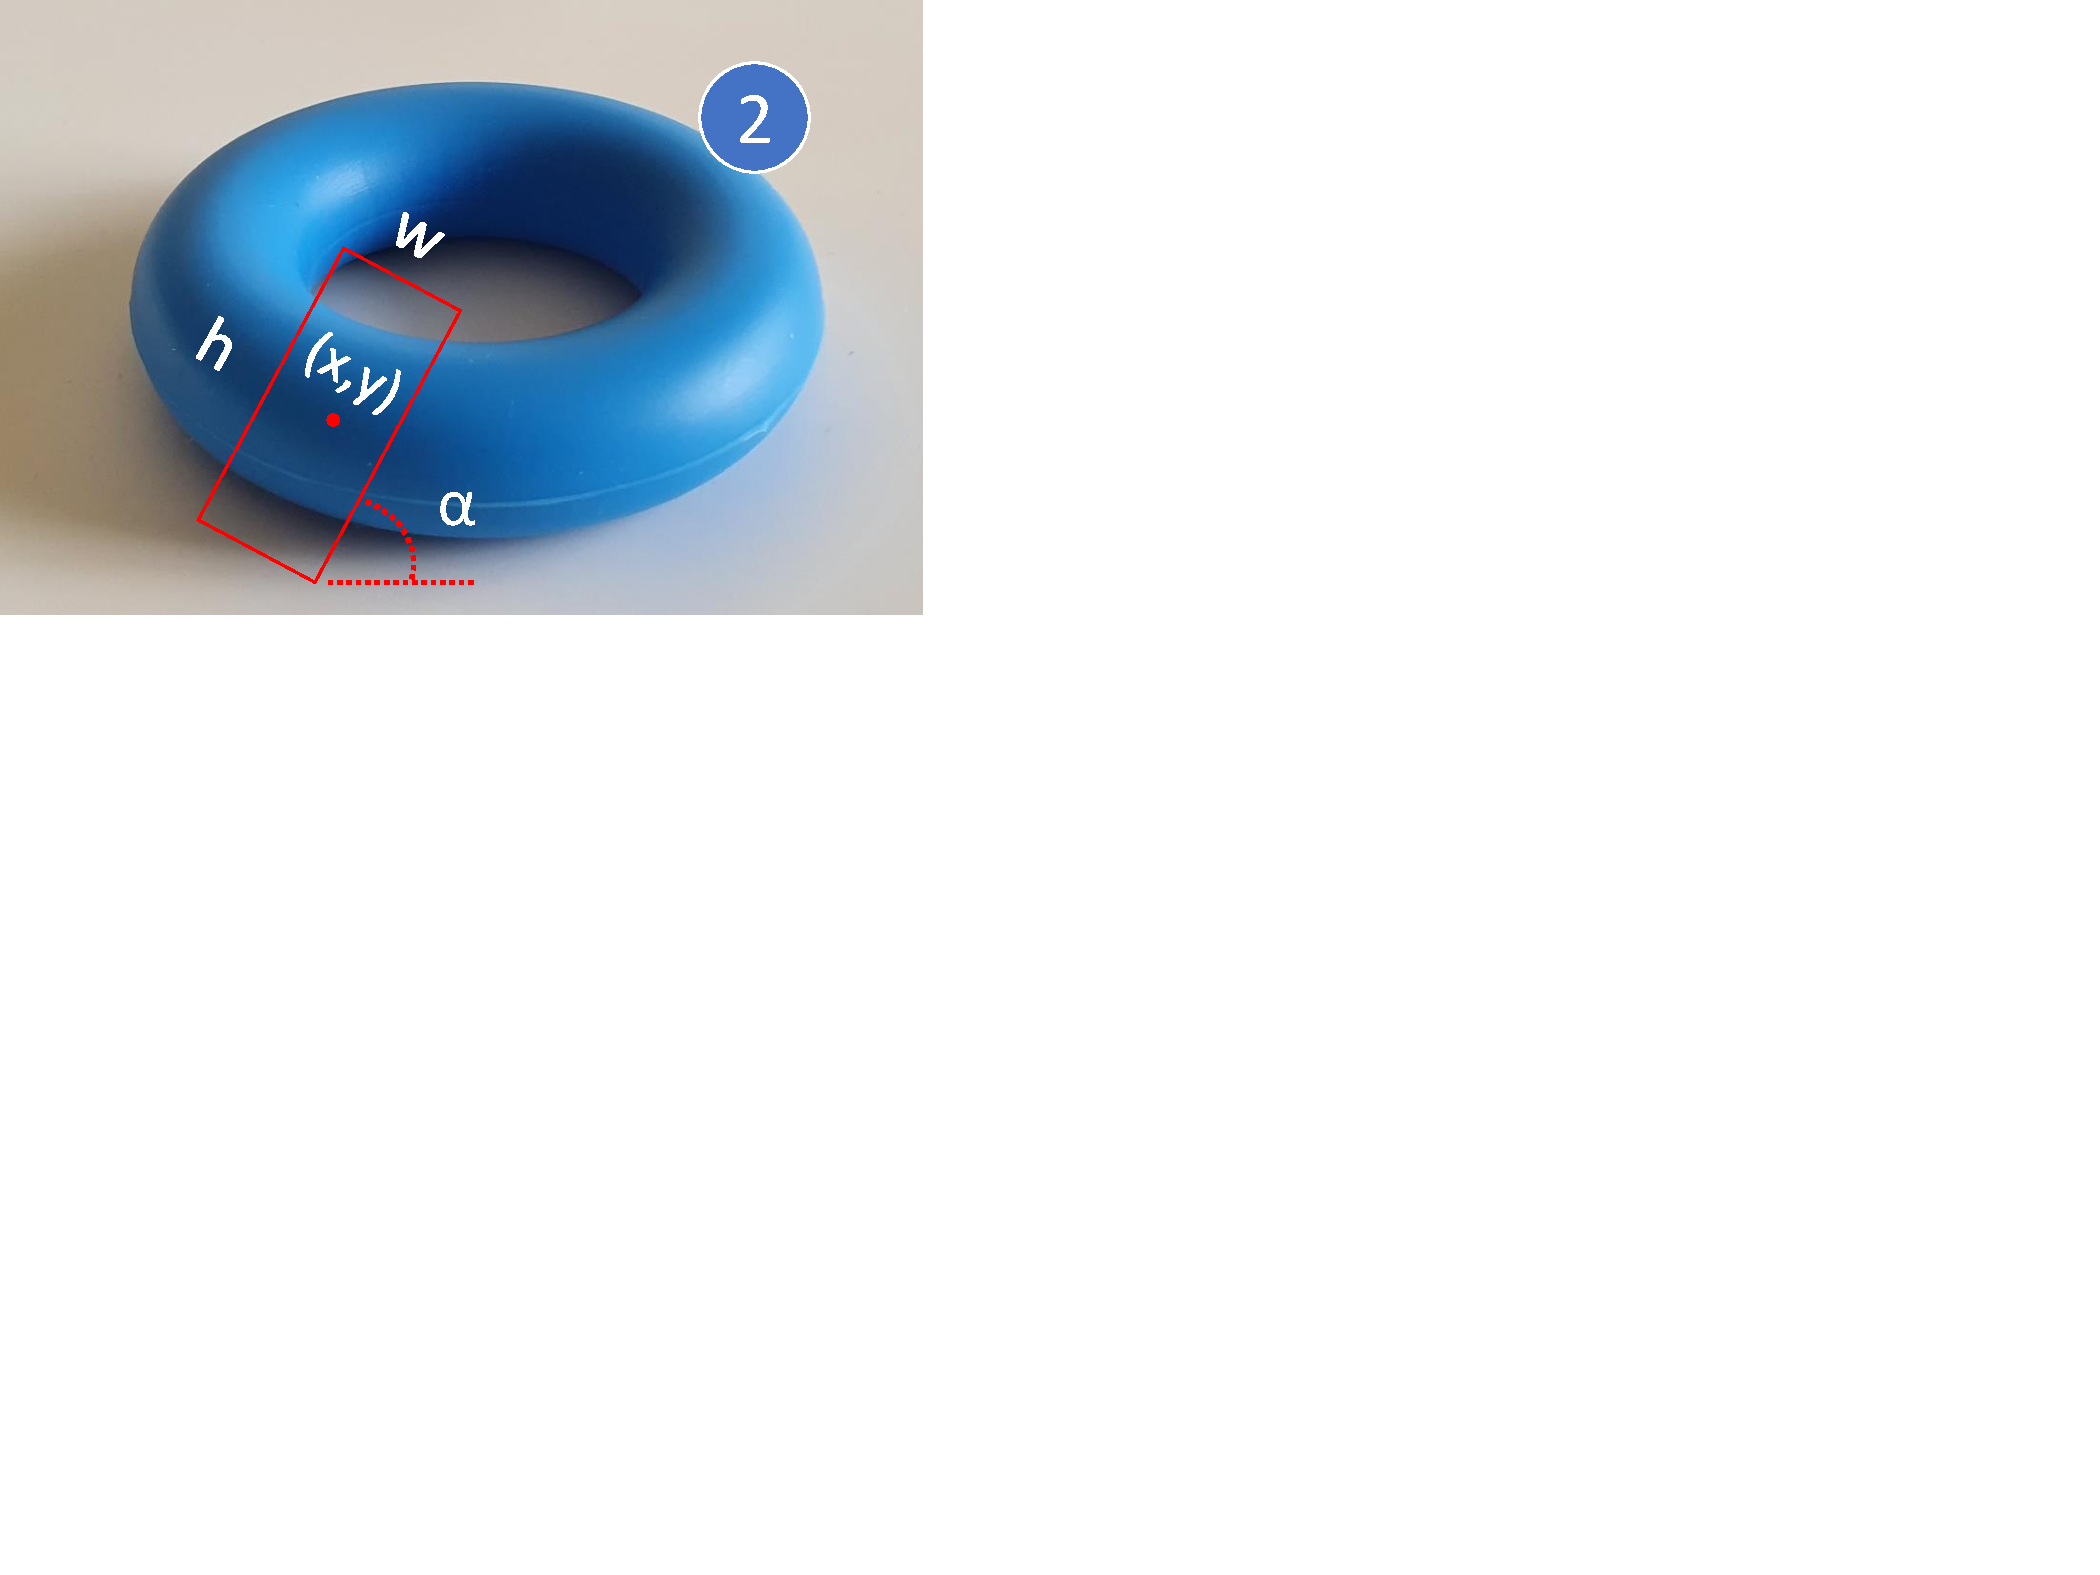
\includegraphics[trim={19mm 162mm 215mm 8mm},clip,width=1\linewidth,angle=0]{Cap2/Figuras/rec_rep.pdf}
				%\caption{Partial form fit combined with clamping force.}
				%\label{fig:g2}
			\end{subfigure}
			\hfill
			\begin{subfigure}[c]{0.45\textwidth}
				\centering
				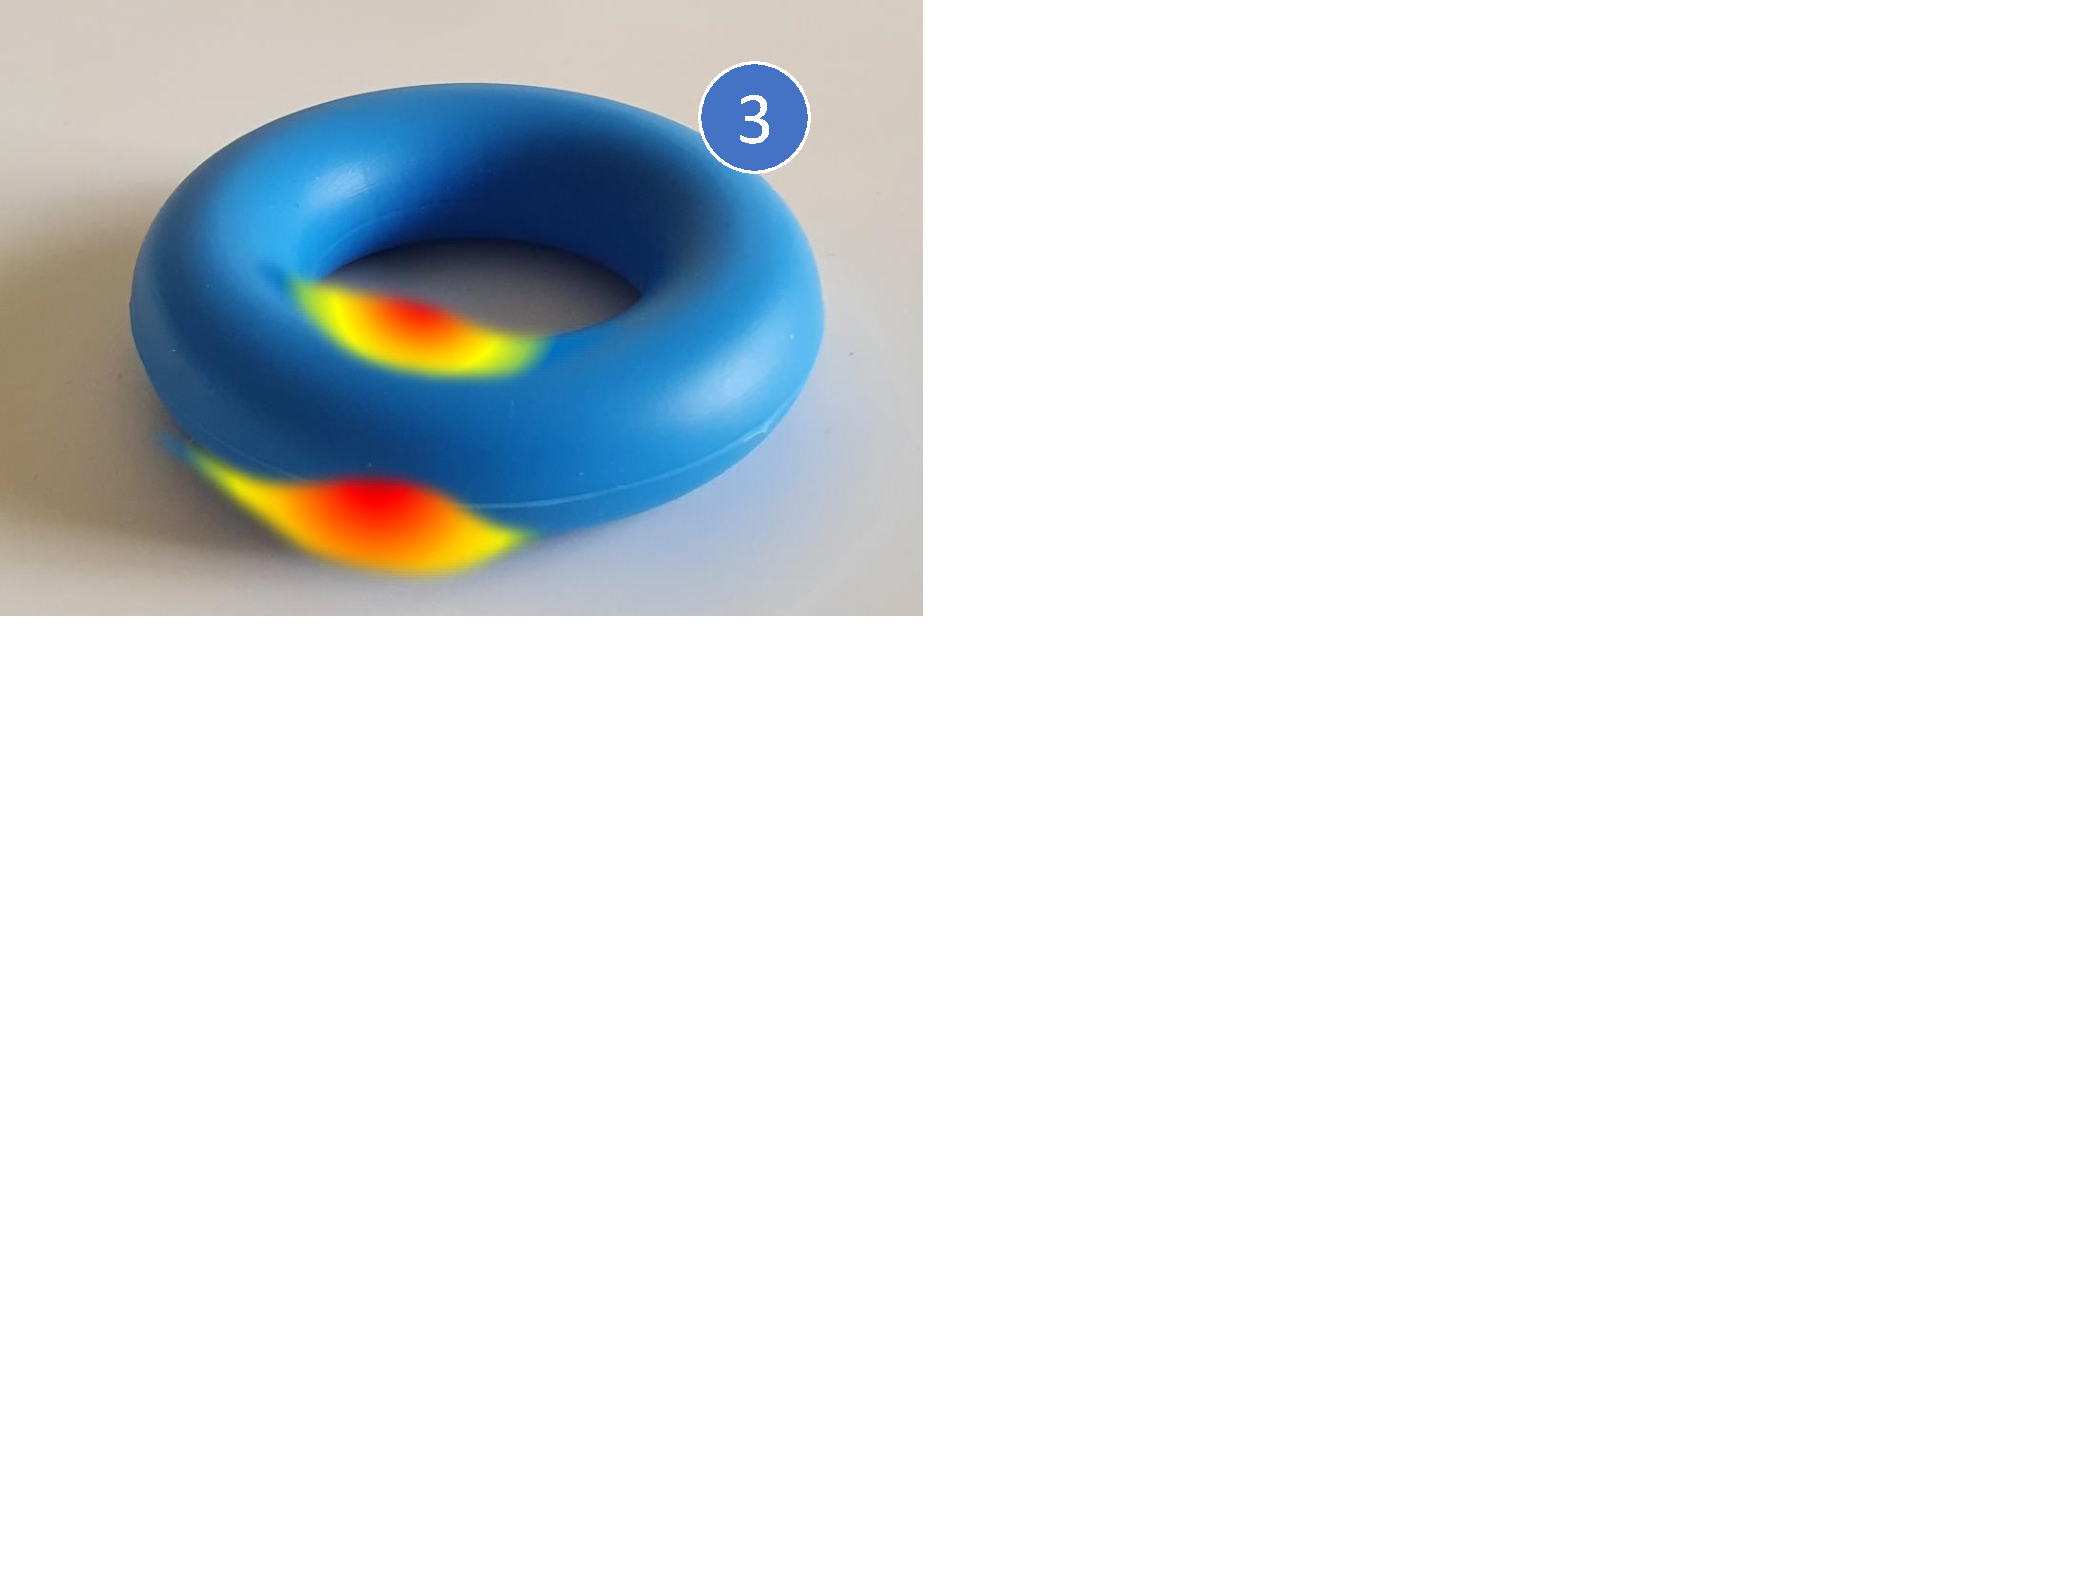
\includegraphics[trim={19mm 162mm 215mm 8mm},clip,width=1\columnwidth,angle=0]{Cap2/Figuras/myBeliefMap.pdf}
				%\caption{Pure force closure.}
				%\label{fig:g3}
			\end{subfigure}
			\hfill
			\begin{subfigure}[c]{0.45\textwidth}
				\centering
				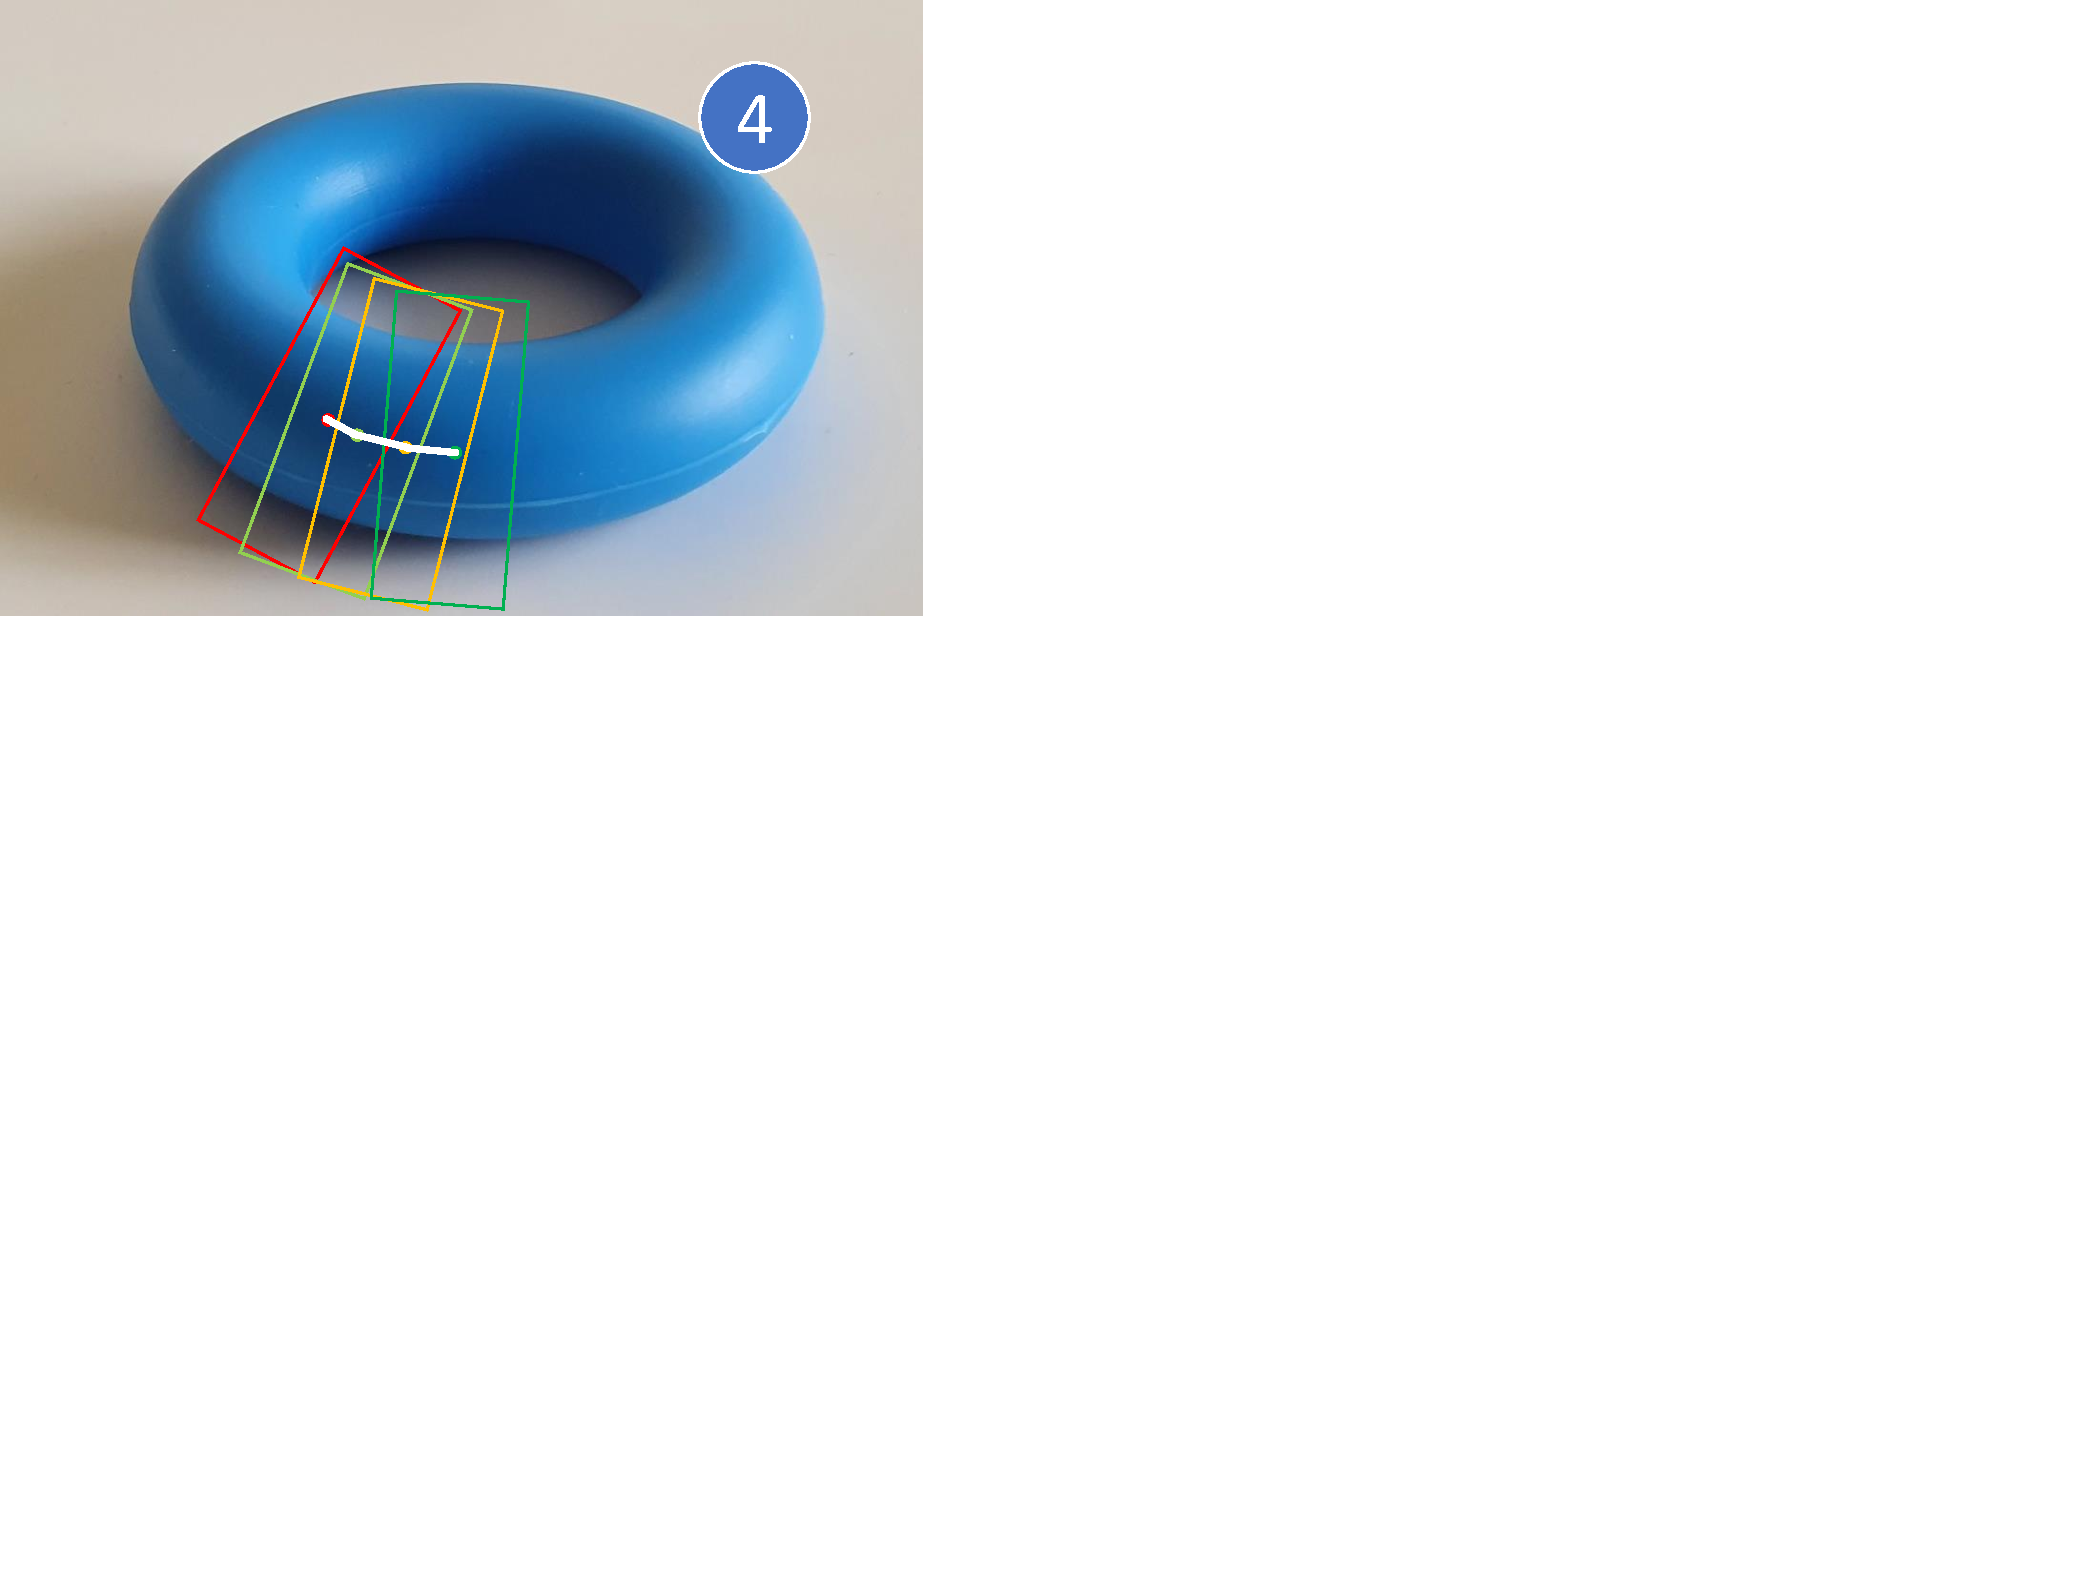
\includegraphics[trim={19mm 162mm 215mm 8mm},clip,width=1\linewidth,angle=0]{Cap2/Figuras/myGraspPath.pdf}
				%\caption{Holding with vacuum air (pneumatic force closure).}
				%\label{fig:g4}
			\end{subfigure}
		\end{tcolorbox}
		\caption{Grasping representation in 2D images. Grasping point (1) describes a grasping position $(x,y)$ without any physical considerations, while the rectangle representation (2) also represents the gripper's width ($w$), height ($h$), and orientation ($\alpha$). The grasping belief map (3) models a spatial uncertainty in a grasp distribution fashion. The grasping path (4), described by a white line, leads the prediction of several possible rectangle grasp candidates.}
		\label{fig:exemples_rep}
	}%end of resize box      
\end{figure}



%\begin{figure}[h]
%    \centering
%    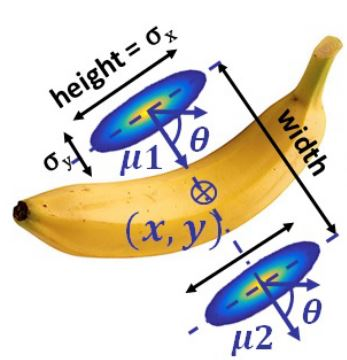
\includegraphics[scale=0.5]{Cap2/Figuras/grasping_belief_map.JPG} 
%    \caption{Grasping Belief Maps and Grasp Path.}
%    \label{fig:grasp_belief_grasp_path}
%\end{figure}

% \begin{figure}[h]
%     \centering
%     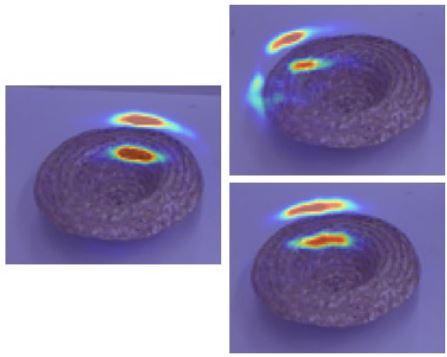
\includegraphics[scale=0.75]{Cap2/Figuras/grasping_belief_map2.JPG} 
%     \caption{Grasping Belief Maps~\cite{Ghazaei2019}.}
%     \label{fig:grasp_belief_map}
% \end{figure}

% \begin{figure}[h]
%     \centering
%     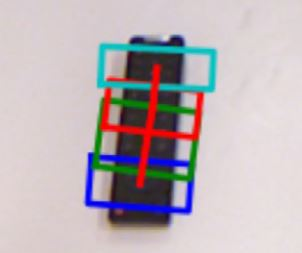
\includegraphics[scale=.5]{Cap2/Figuras/grasp_path.JPG} 
%     \caption{Grasp Path~\cite{Chen2019}}
%     \label{fig:grasp_path}
% \end{figure}

%\subsection{Discussion}
%\label{cap2:related_work:sec:grasping_representation:subsec:discussion}


As it is possible to see in this section, grasping representation is an essential phase in grasping planning. The mathematical formulation and description, such as wrench space analyses, antipodal restriction, $\epsilon$-value, and volume metrics are the basis for understanding physical phenomena between the active-pair interaction, e.g., basis widely used in 3D model grasping representations (3D-sensing and CAD simulations). However, these mathematical description techniques showed to be limited by several factors, e.g., high complexity implementation according to application demands and the necessity to know the gripper and graspable object characteristics. Therefore, these approaches typically work well only in specific cases.  

\begin{tcolorbox}[every float=\centering, drop shadow, title= Jacquard threshold]
	
	The Jacquard threshold also referred to as the Jacquard index, is commonly used as a quality metric for grasping predictions. The mathematical formulation is defined by $Area(G\cap G^*)/Area(G\cup G^*)$, where $G$ and $G^*$ are the predicted and the ground-truth grasping rectangles, respectively. It is restricted to rectangle grasping representation which is widely used by two-finger grasps. It is important to notice that this approach can lead to miss concept conclusions since the high Jacquard index is not completely related to grasping success, e.g different rectangle orientations can have the same intersection region, therefore the same Jacquard value, and lead to unfeasible grasps. Thus, it is common that this metric has complementary analyses in several works.
	
	\vspace*{1ex}
	
	\centerline{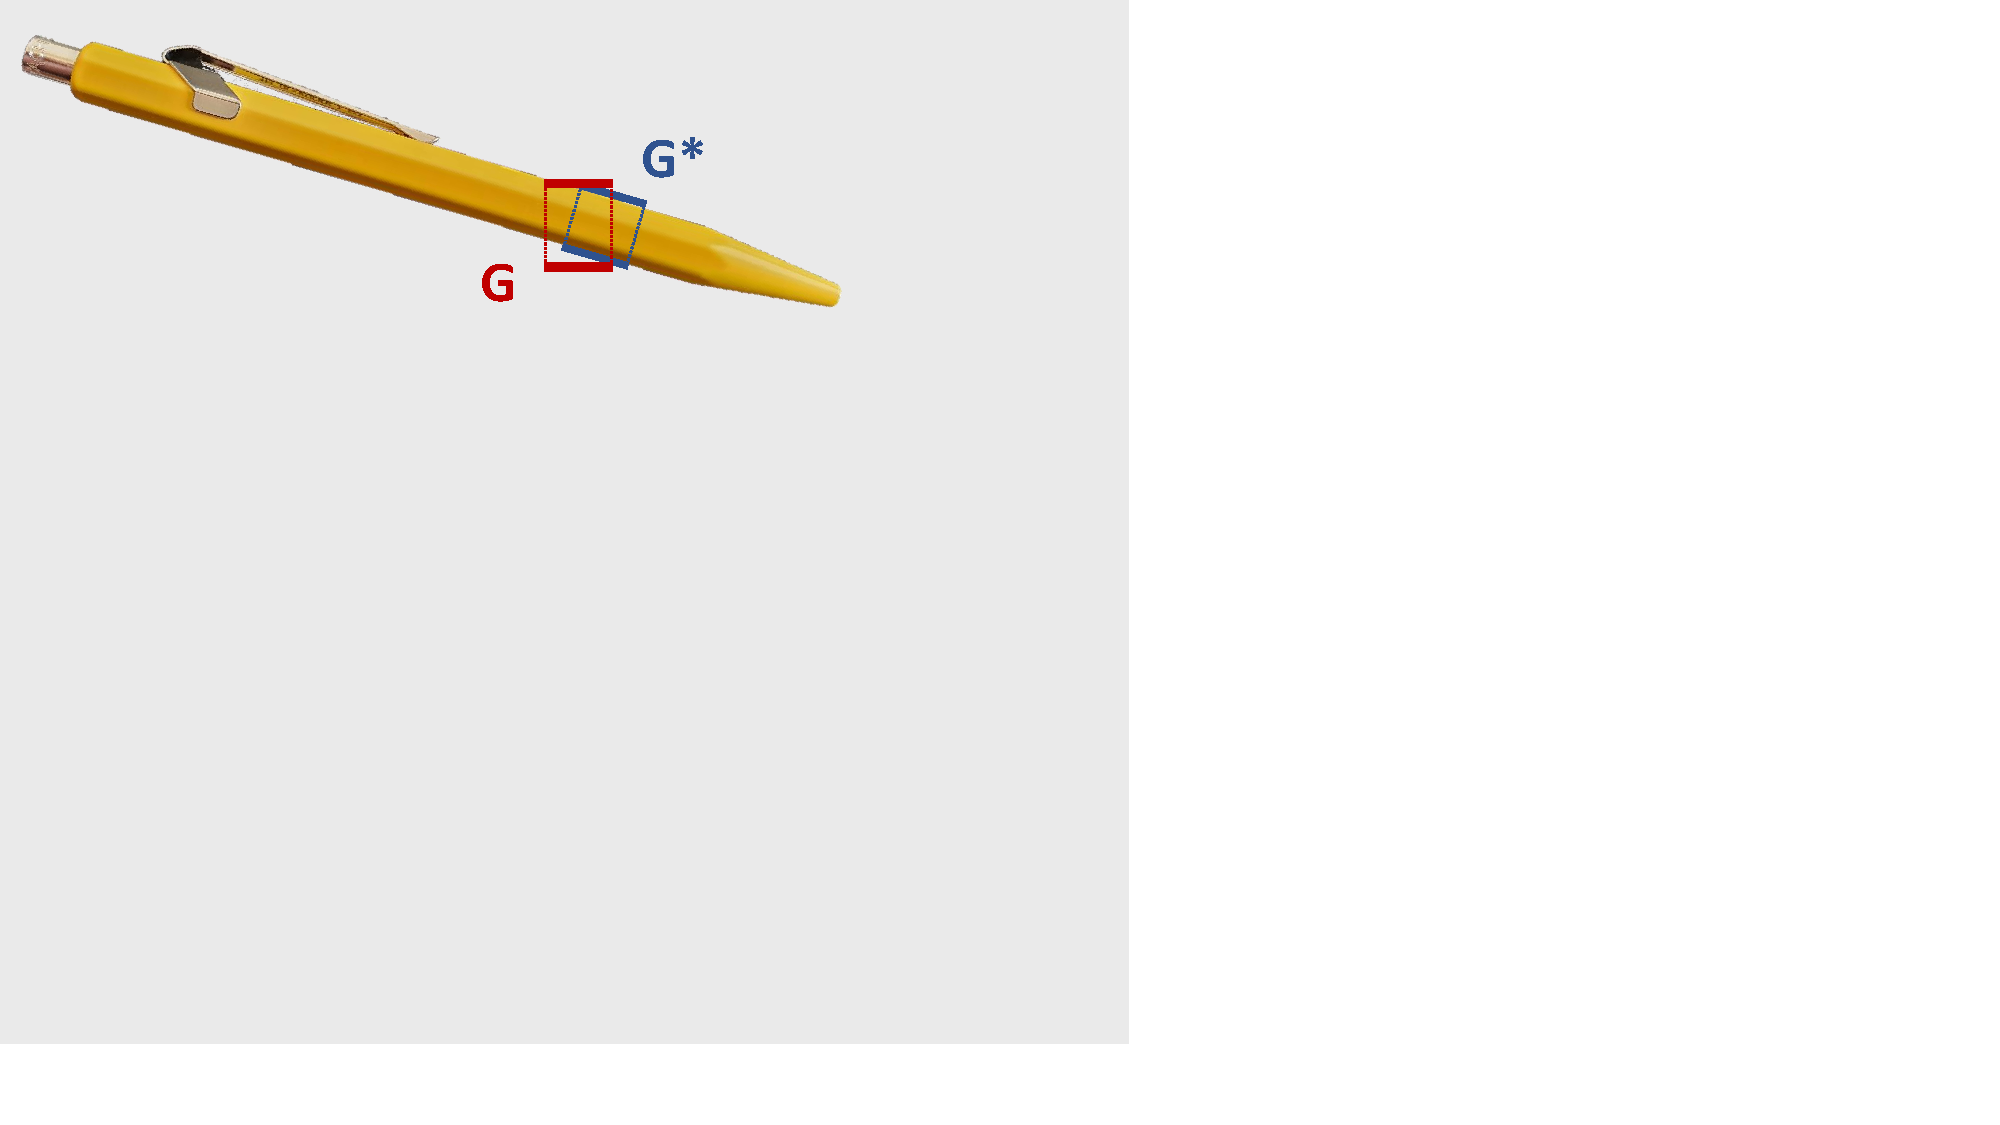
\includegraphics[trim={0cm 12.5cm 17cm 0cm},clip,width=.65\linewidth,angle=0]{Cap2/Figuras/pen_jacquard.pdf}}
	\captionof{figure}{Jacquard threshold representation.}\label{fig:pen_jacquard}
\end{tcolorbox}

The 2D image grasping representation, as already stated, has a lack of fully physical grasping representation. This factor is prominent in point representation since the grasping is only described by its spatial coordinate. Differently, the rectangle representation also includes gripper properties, e.g. finger's width and height, but does not consider friction or any spacial uncertainty, such as the belief map's. The Grasp Path could also be an alternative since it guides several grasp hypotheses to contour the limited space search problem.

It is important to note that, in numerous proposals, the discussed cases are used, and the gripper structure generalisation is not considered (typically, only two fingers are investigated), showing the complexity of this task.

Heretofore, to the best of the authors' knowledge, the most promising representation is formulated by DexNet dataset proposed in~[32-36]. The DexNet is constituted by 3D CAD models labelled with robust grasps for two-finger and suction grippers, i.e., the database was build considering analytical methodologies, iterative algorithm, and simulation interactions. They also included bin-picking and ambidextrous policies. This leads to the idea that the human grasping intuiting is more complicated than only visual representation.


% Ghazei et  al. ideia could be a start ideia to solvenot rigid objects.

\section{Robotic Grasping Approaches}
\label{cap2:related_work:sec:grasping_approaches}

Since the advent of robotic operations, numerous proposals explore the grasping solution idea, from analytical to deep learning approaches. In summary, analytical methods showed to be the first solution to several proposals that achieved exciting results in specific cases. They also formulate the basis used in recent days. However, the main problem is the object grasping generalisation and complexity rise according to the application demand. Currently, the computer science field advances led to machine learning usage that shows to be a potential method to deploy effective grasping solutions, until now not reached but with promising results. 

Therefore, the present section is an effort to categorise these strategies over the years and build a structured basis for new studies. This section is organised as follows: first, the analytical methods are explored in Section~\ref{cap2:related_work:sec:grasping_approaches:subsec:analytical_review} following by the data-driven grasping policies, Section~\ref{cap2:related_work:sec:grasping_approaches:subsec:learning_review}. As the deep learning methodology has been the study-case of several state-of-art proposals, this data-driven policy subcategory is presented apart in Section~\ref{cap2:related_work:sec:grasping_approaches:subsec:deep_learning_review}.

\subsection{Analytical Methods}
\label{cap2:related_work:sec:grasping_approaches:subsec:analytical_review}

% A few decades ago, the study of grasp planning was focused on analytical methods. This class of grasping is based on a problem's mathematical model considering the kinematics and dynamics formulations and, strongly depends of the know-how's grasping issue of the specialist, since it is hand-designed methodology. This strategy proved to become complicated, even in the formulation or in computer processing. The challenges arise quickly when more refined is the modelling. Therefore, it is possible to find a significant number of papers that solve specific cases of grasp using the mathematical modelling of the grasp issue. Typically these works are focused in the force- and form-closure properties, wrench space analyses, contact's/friction's equilibrium and stability study. 

% Nguyen [1] proposed and proved some definitions and propositions well suitable and accepted by the actual literature, regarding the creation of three fingers and two fingers gripping contacts in the case of polyhedral and polygon objects. Besides, he proposed an algorithm to perform force closure grasp in these conditions. Nguyen also presents in [2] the development of an algorithm to create a set of stable grasps. In the paper [3], the author proposes an extension of the Nguyen's after a review of analytical analyses, definitions, and propositions while Li et al. [4] offer a different approach, with new analytical definitions, to calculate a three-finger force-closure grasps of 2D objects extending to 3D objects. 

In the beginning, grasping planning was focused on analytical methods. This grasping class is based on a problem's mathematical model considering the kinematics and dynamics formulations. Well-accepted and suitable definitions and propositions regarding form- and force-closure grasping were first explored by~\cite{diziouglu1984mechanics,Nguyen1987_1,Nguyen1987_2}. Subsequently, several proposals extend its grasping stability analyses like~\cite{bicchi1995closure, ponce1995computing, li2003computing} and
the firsts algorithms were proposed, as~\cite{liu1999qualitative,liu2000computing,ding2000computing}. The readers are encouraged to review~\cite{murray1994mathematical,prattichizzo2016grasping} for an embracing grasping analysis.

%TODO: maybe remove the part bellow
% Liu presents a qualitative and a grasp optimized force-closure grasping algorithm in~\cite{liu1999qualitative}. Here, the qualitative analyses are based on the convex theory about the wrenches and are solved with a linear programming method. This paper has an interesting algorithm to evaluate and define the wrenches (the values of the force according to the friction cone) to perform a force-closure but does not estimate the position of the fingers. Trying to formulate a solution to a n-finger gripper, Liu in~\cite{liu2000computing} also proposes an algorithm to estimate all force-closure grasps of an n-finger gripper on a polygonal object. Namely, it defines regions on space to allow a force-closure grasp. Results were evaluated under analytical programming; it was not evaluated using neither a real nor a simulated scenario. The proposal is only for polygonal objects and considers the force-closure analyses taking into account the places of the fingers without defining where to put the finger. Another approach is presented by the authors of~\cite{ding2000computing} who create an optimization algorithm where the position of n-m fingers to perform a force closure grasp to 3D polygonal objects is calculated a priori. 

The analytical methods are applied in specifics cases, with the complexity rising according to the applications' demand. The disparity in mathematical modelling and the real operation is also an issue. Complete and generic analytical grasping solutions are presented by~\cite{liu2004complete,el2009computing} and elucidate these problems. \citeauthor{liu2004complete}~\cite{liu2004complete} propose a complete analytical solution to find a 3D force-closure grasp, frictional or friction-less, for any type of object, including the one with a curved surface. The algorithm combines a local process with a recursive strategy of problem decomposition. First, it inserts n-contacts on the object and recursively tries to find a convex hull that includes the origin. When the search finds a local minimum, the algorithm sets the recursive decomposition method decomposing the problem in sub-problems. Results are analysed over numerical examples without a completely guarantee to find a feasible grasp; an issue is a computational complexity that needs to be evaluated according to the number of contacts used.

\citeauthor{el2009computing}\cite{el2009computing} addressed robust force-closure grasps for generic objects with n-finger hands. To achieve the goal, authors randomly generate $n-1$ fingers position and define the last finger position using the strictly negative linear combination of one of the first generated $n-1$ fingers wrench basis. In this way, the authors reached a faster algorithm, to the detriment of the success rate.

It is important to note that some analytical approaches only aim at estimating the stability of suitable grasps, sometimes called grasping synthesis. However, it is also necessary to determine the best grasp to perform the task. Some analytical methods treat this step as an optimisation problem (\cite{Ciocarlie2009,rakesh2018optimizing}) of some quality measurements. As listed by \citeauthor{Roa2014}~\cite{Roa2014}, a quality measurement can be categorised based on the contact points' position and the hand configuration. An extensive review of these quality methods is presented in~\cite{Roa2014}. These measurements define the grasp analyses optimisation that, in several cases, do not guarantee the grasp determination because of the local minima problem.


\citeauthor{Ciocarlie2009} proposed in~\cite{Ciocarlie2009} to embed the ``Very Fast Simulated Re-Annealing''~\cite{ingber1988}~\cite{kirkpatrick1983} optimisation algorithm, into \textit{Graspit!} simulator~\cite{AndrewT2004}, a widely used grasping planning environment~\cite{morales2006integrated, carvalho2020}. With a 3D pair-wise model, this algorithm tries to reduce the distance of the gripper's contact points and the object's surface evaluating wrist pose and gripper/hand posture. As discussed by \citeauthor{Ciocarlie2009}~\cite{Ciocarlie2009}, the hand posture is defined by \textit{eigengrasps}, a subspace of movement based on how human-generated hand postures. The \textit{eigengrasps} reduces the hand's DOFs based on how humans select appropriate grasps and hand postures. Studies~\cite{Ciocarlie2009,Santello2002} show that humans simplify, unconsciously, the problem with a pattern in the movement. 

Besides the interesting results, the discussed methods demand some unfeasible application efforts, e.g., the optimisation's convergence time could limit the run-time grasping decision process. Thus, the strategy to divide the grasping planning into offline (grasping synthesis) and run-time processes (grasping selection) are used~\cite{carvalho2020}. Typically, the offline procedure generates a list of grasp candidates. The run-time selects the best grasp (under task-oriented capabilities) after matching the sensing data to a dataset. The major problem of these techniques is to know the objects' shape and the gripper's structure. Therefore exceed grasping of novel objects based on already known ones is not possible. This evaluation incorporates the sensing step into grasping planning rather than only perform object localisation and recognition.

%\begin{figure}[h]
%    \centering
%    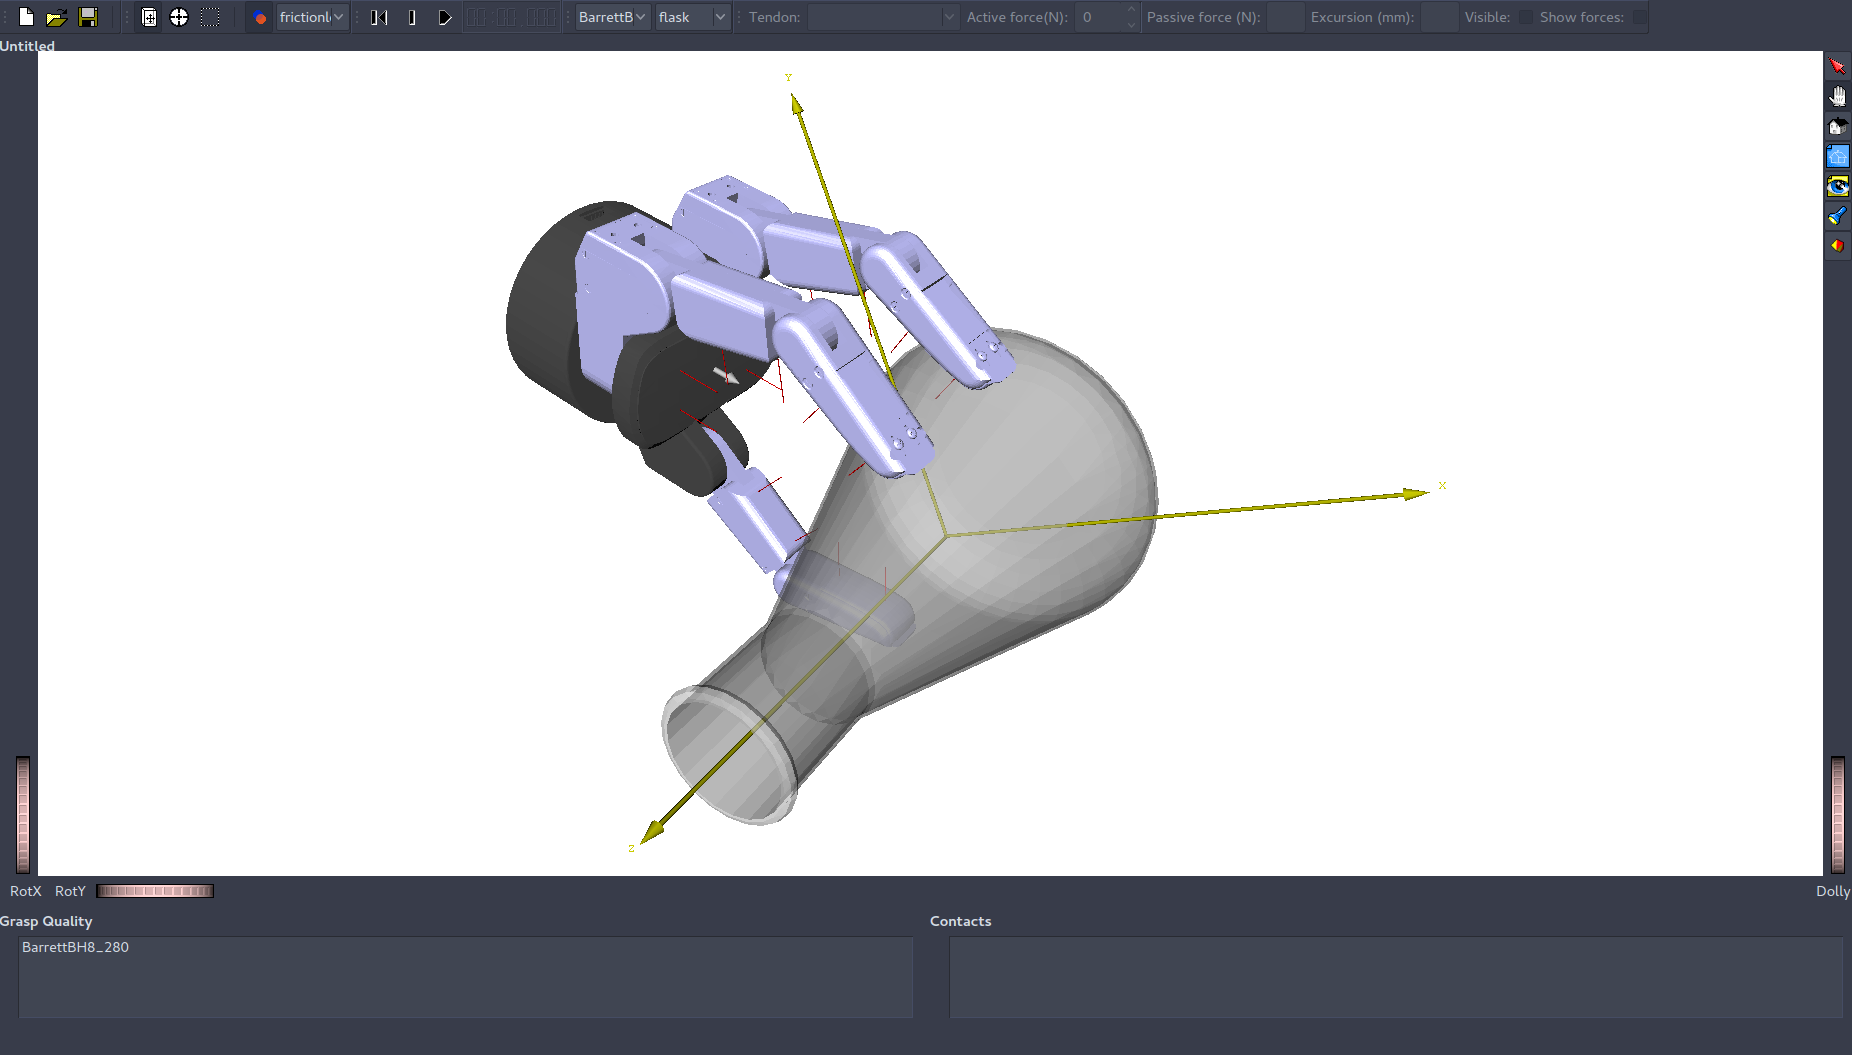
\includegraphics[trim={0 0 0 0},clip,width=1\columnwidth,angle=0]{Cap2/Figuras/graspit5.png} 
%    \caption{``Graspit!'' simulator.}
%    \label{fig:graspit}
%\end{figure}

Once knowing how to grasp spheres, cylinders, cones, and boxes with analytical methods,~\citeauthor{Miller2003}~\cite{Miller2003} investigate the idea to approximate an object to these primitive shapes. \citeauthor{Jain2016} did the same~\cite{Jain2016} by using the point cloud directly. In this context, some approaches use object model decomposition in a set of primitives and execute the ``grasping by parts''. Therefore, the grasping synthesis is simplified, and heuristics methods, associated with analytical approaches as quality control, are proposed. Not only the shape definition is used, but the decomposition tree with superquadrics shapes~\cite{Goldfeder2007}, Reeb graph~\cite{Aleotti2012}, and Medial Axis Transformation~\cite{Przybylski2011} methods are examples trying to solve the related issue. 


% These are the cases of primitive shape, superquadratic and Medial Axis Transformation decomposition methods of~\cite{Miller2003}, \cite{Goldfeder2007}, and  \cite{przybylski2011planning}. Decomposing an object point cloud in primitives and creates two-finger gripper grasps candidates [5] is also an alternative to the previously unknown of the object shape. The grasping by parts is also present in learning policies.

% Verificar se é necessario o seguinte paragrafo.
As discussed in the presented section, the analytical approach has a list of issues that can be summarised as high modelling complexity; high computational complexity; practical inconsistencies; and restricted assumptions. Therefore, the use of learning methods has gained attention, and its development is growing. This fact is verified by the crescent number of papers regarding this theme.

\subsection{Data-Driven Grasping and Learning Policies} 
\label{cap2:related_work:sec:grasping_approaches:subsec:learning_review}

As presented in Section~\ref{cap2:related_work:sec:grasping_representation}, in robotic grasping there is a lack of full representation of the input data, i.e., a partial data representation structure. For instance, a 2D image cannot map the truly grasping interaction, while the simulation could reduce this problem in the loss of applicability. Modelling all physical interaction and noise is unfeasible. However, this issue is not restricted to robots but also presented in humans. Humans can plan to grasp using a stereo-based image with eyes and based on previous experience~\cite{castiello2005neuroscience}. This simple motivation lead studies about learning methodologies to supply these demands, and some pioneer studies can be reviewed in~\cite{Oztop2001, Wheeler2002, Rezzoug2002}.

Indirectly, the optimisation grasping techniques use data or previously known interaction to find a possible solution or refine it~\cite{roa2009finding}. Therefore this kind of methodology can also be included in the data-driven category. However, looking for structured categorisation, this section will only discuss methods regarding classification and machine learning algorithms.

\citeauthor{Pelossof2004}~\cite{Pelossof2004} explore the application of \ac{SVM}, trying to find a regression function to build a map between object shape, grasp parameters, and grasp quality. The authors face the problem of grasp representation in \ac{SL} methodology. Therefore, it was proposed the use of the superquadric objects since these are easily characterised. This approach limits the grasping generalisation only to novel superquadric objects. The ``GraspIt!'' simulator was deployed to generate the database and propose as future work the superquadric combination to characterise more complex objects, later studied by~\cite{Goldfeder2007}. The complexity of feature extraction, while considering different grippers, was also a pioneer study by \citeauthor{dini2000planning}~\cite{dini2000planning}, where a classic Neural Network was proposed to classify an object-agnostic grasping qualitatively. A more recent work~\cite{tenPas} use \ac{SVM} to classify antipodal grasping directly from a point cloud and without recognising it. This paper also evaluates the performance in a densely cluttered environment. The same methodology was used in~\cite{Mahler2017b} but with a grasping proposed database. \citeauthor{Mahler2017b}~\cite{Mahler2017b} also evaluate the use of the Random Forest \ac{SL} algorithm motivated by the work of~\cite{seita2016large}. %However the results do not achieve state-of-art success rates. 

\citeauthor{Saxena2008}~\cite{Saxena2008} was one of the first to explore the supervised grasping learning technique and target object 2D image-based features. They were also motivated by the fact that human object recognition is not related to grasping~\cite{goodale1991neurological}. For this, the authors propose using logistic regression to find grasping point representations and were able to grasp a variety of novel household objects with a success rate of 87.8\%. Based on this, \citeauthor{Jiang2011a}~\cite{Jiang2011a} proposes the use of a two-stage \ac{SVM} classification to detect rectangular grasping contesting the point representation (see Section~\ref{cap2:related_work:sec:grasping_representation}). The first stage is faster and less accurate, while the second stage is more accurate with complex feature detection. Their studies motivate the grasping by an image that later evolves to deep learning policies (Section~\ref{cap2:related_work:sec:grasping_approaches:subsec:deep_learning_review}).

\citeauthor{Trottier2017}~\cite{Trottier2017} use the rectangle strategy, RGB-D images, and \ac{DLSR}, showing a different strategy to \ac{SL} procedure. The authors propose several architectures trying to avoid the big dataset needed for deep learning policies (discussion in Section~\ref{cap2:related_work:sec:grasping_approaches:subsec:deep_learning_review}). They achieved a state-of-art grasping detection rate, but the processing time was not qualified to perform the grasping. %It is also possible to teach a robot grasping by demonstration, in a \ac{LbD} fashion, as related by XXXX. XXX

The \ac{RL} applied to robotic grasping is the focus of studies~\cite{Bernd2002,BaierLowenstein2007, boularias2015learning, platt2007learning} that try to avoid the \ac{SL} approaches shortcomings, e.g., the time-spend to build a labelled database and the limitation of grasping performance according to the supervisor/teacher ability to interpret the physical problem. Typically this class of algorithms is based on trial-and-error approaches focusing on maximising a cumulative reward function. This concept allows an object-agnostic grasping procedure without environment restrictions modelling. However, the major drawback is the time-consuming learning experiments. \citeauthor{boularias2015learning}~\cite{boularias2015learning} use the strategy to push the objects before grasping them in clutter scenes, which was modelled as a \ac{MDP}. A kernel-based \ac{RL} methodologies were implemented, showing that pushing movements can improve grasping performance. Instead of using visual information, \citeauthor{platt2007learning}~\cite{platt2007learning} investigates how to grasp using the contact relative motion model, i.e., using a force sensor as feedback, the algorithm tries to increment small displacement of the finger until reach grasp stability. Modelling it as a \ac{POMDP},~\cite{platt2007learning} tries to solve the optimal control problem using~\ac{RL} methodologies. First, a simulated \ac{RL} was used, which was later transferred to the real robot. This approach is more related to a refined grasping procedure than a grasp synthesis since an initial random grasping point needs to be a priori estimated.

Nowadays, the \ac{SL} and  \ac{RL}  methods were guided to \ac{DL} methodologies based on the promising results of deep architectures applied in robotic task generalisation. Therefore, it is possible to define a distinctive category that will be presented in Section~\ref{cap2:related_work:sec:grasping_approaches:subsec:deep_learning_review}, the deep learning grasping.


%TODO: ler mais papers daqui... Learning: LbD; RL; SL; UL ....

\subsection{Deep Learning Grasping Policies}
\label{cap2:related_work:sec:grasping_approaches:subsec:deep_learning_review}


The new deep learning policies and deep network architectures have leveraged computer vision detection tasks, as the object recognition problem proposed by ImageNet Large Scale Visual Recognition Challenge~\cite{imagenet_challenge}. In this field, the advent of deep \ac{CNN}~\cite{krizhevsky2012imagenet}, and the constant improvement of its architecture shown promising results. These results have been drawn the attention of robotic researchers that seek to apply the generalisation capability of these networks in the grasping issue, as can be seen by the competitor's proposals of Amazon Picking Challenge~\cite{amazon_challenge}.

\citeauthor{Lenz2015}~\cite{Lenz2015} was one of the first to investigate the \ac{DL} in grasp planning. In their proposal, a grasp rectangle~\cite{Jiang2011a} is elected after a two-stage cascade detection learning network using RGB-D images. The first layer, less accurate, is responsible for learning a large number of direct features from the view, and the second layer selects the best grasp position using these features. The input image is gathered using a sliding window technique. However, this strategy compromises the real-time application, as reported by
~\cite{Redmon2015, Guo2017,Chu2018}. \citeauthor{Lenz2015}~\cite{Lenz2015} verified that the \ac{DL} improve the learning process since a hand-engineering feature modelling was not needed. Another precursor \ac{DL} work was proposed by \citeauthor{Redmon2015} in~\cite{Redmon2015} which applied the AlexNet~\cite{krizhevsky2012imagenet} \ac{CNN} architecture to grasping prediction.  \citeauthor{Redmon2015}~\cite{Redmon2015} explored the Transfer Learning concept between \ac{DL} applications, latterly used by works~\cite{Kumra2017,TenPas2017, Chen2019,Mahler2017d,Zeng2019,Chen2020}, and verified that this approach supports the training process preventing over-fitting due to the limited labelled database size. Their proposal uses a complete RGD image to direct regression to rectangle grasp. The strategy of replacing the blue channel with depth is also verified in subsequent works~\cite{Kumra2017,Chen2019,song2020novel} that adapt the image classification \ac{CNN} architectures to the grasping problem. The authors affirm that adding an extra channel in these architectures avoids the pre-training phase with the image classification dataset. Therefore, the grasping architecture was pre-trained with object classification of~\cite{imagenet_challenge} and also evaluated by the hypothesis to classify an object before grasping it. The authors achieved an almost $85\%$ of detection success rate (see Table~\ref{tab:met_state_of_art}), however when the proposal is exceeded to real grasping a reduction in the efficiency is related, as can be verified by the results achieved in~\cite{Watson2017} and~\cite{Chu2018}.

After the advent of ResNet \ac{CNN} architecture~\cite{he2016deep}, \citeauthor{Kumra2017}~\cite{Kumra2017} propose its use in grasping in two different modalities: uni-modal with direct RGB or RGD data, and multi-modal with RGB and three-dimensional depth data, therefore two ResNet networks. In both cases, the ResNet layer was responsible for extracting the features that were classified as good grasping by a fully connected layer. This multi-modal strategy is also verified in papers as~\cite{Guo2017}. However, \citeauthor{Guo2017}~\cite{Guo2017} use tactile data motivated by the fact that the grasping is not only a classification image-like problem.  It was expected to model the grasp stability during the training process indirectly. With a deep visual network and a deep tactile network, the hybrid architecture achieved an $89\%$ detection success rate. The practical grasping performance was tested by \citeauthor{Chu2018} in~\cite{Chu2018} achieving a success rate of $81\%$ (see Table~\ref{tab:met_state_of_art}). \citeauthor{Chu2018}~\cite{Chu2018} also proposed the use of  ResNet and VGG-16 \ac{CNN} architecture with candidate regions to a focused feature search (motivated by \ac{RPN}). With this approach, the authors achieved interesting detection rates with practical evaluation, see Table~\ref{tab:met_state_of_art}. 

The ResNet is also used by \citeauthor{Ghazaei2019}~\cite{Ghazaei2019} in a \ac{FCN} architecture which, instead of finding a regression from RGB images to rectangle grasp, direct output a Grasp Belief map (see Section~\ref{cap2:related_work:sec:grasping_representation}). However, to evaluate and train their network, it was used the \ac{CGD} which caused~\cite{Ghazaei2019} to ``translates'' the belief map in rectangle grasping, compromising the truly potential evaluation. Other examples of deep \ac{CNN} applied to the grasping problem is the LeNet of~\cite{TenPas2017} that use direct Point-Clouds of the scene to estimate feasible antipodal grasps, and the DarkNet53 (from YoloV3)~\cite{Chen2020} used to estimated the grasp path discussed in Section~\ref{cap2:related_work:sec:grasping_representation}. 

It is possible to notice that a better grasp success rate is more dependent on a complete grasping modelling than only the Deep Network architecture strategy. This fact can be seen by the DexNet project's design which confirms that the grasping planning is a more complex task than only a classification image-like problem. \citeauthor{Mahler2016} start the DexNet project~\cite{Mahler2016} designing an algorithm to create a more reliable database called DexNet 1.0. This database, interactively generated, is composed of a set of parallel-jaw grasps associated with the object's 3D model. Each grasp is labelled with a probability of force closure under uncertainty in object pose, gripper pose, and friction coefficient. In the following works, the database evolved, including: scenario constraints, as planar base surface; different scene points of view; bin-picking and dense clutter scenarios; and ambidextrous policies to select the appropriate gripper (suction or two-finger). With the DexNet, a \ac{GQ-CNN} was proposed to select and define a robust grasp configuration in single object grasping and bin-picking. Nevertheless, the authors encounter challenges in grasp flexible, porous objects and with loose packing.

As shown in this section, building a sufficient size labelled database is the main drawback of \ac{DL} policies. Even though a large database could be available,  assess if the labelled database modelling includes all necessary practical assumptions is difficult. Therefore, some proposals try to overcome this problem by generating data through practical experiments or using \ac{DRL} methodologies. That is the case of \citeauthor{Pinto2015}~\cite{Pinto2015} that generates a proprietary database with 50k tries of random robotic grasping and mapping them to the rectangle database. For the authors, the image ground-truth and the simulated interactions database are questionable. However, their reduced success rate probably is due to their grasping representation simplification. Although their proposal is a \ac{SL}, the authors face a similar problem of \ac{RL} methodologies: the time spent by the database physical try-and-error.

% There exists several \ac{DCNN} architectures that can be applied into a grasping problem, like the discussed AlexNet, ResNet, VGG-16, LeNet~\cite{TenPas2017} and DarkNet53~\cite{Chen2020} and all the results lead to the following interpretation: the grasp representation, Section~\ref{sec:grasping_representation}, and database build plays an important role in grasping success rate. Focusing on that, the DexNet~\cite{Mahler2016, Mahler2017b, Mahler2017d, Mahler2017, Mahler2019} project achieved interesting results including two-fingered, suction grasping, bin-picking, and ambidextrous policies. ...

% {TODO: falar que nao antigiram resultado bon para multiplo objectos e likar com paper do 6DOF}

% Maybe insert images from these papers ...

The authors of~\cite{Zeng2019} propose the direct use of RGB-D pixel-wise to infer, with \ac{FCN}, affordances grasping instead of classical mapping to grasping parameters. In a grasp-first-then-recognise workflow, the authors mapped affordance maps of a discrete set of grasping primitives for suction and two-finger grippers. With this direct approach, as related by~\cite{Zeng2019}, a faster, reliable, and able to learn complex grasping rules was verified. \citeauthor{Zeng2018} also investigate in~\cite{Zeng2018} a Deep Reinforcement Learning methodology to evaluate the synergy between push and grasp, achieving interesting results to adversarial clutter scenarios without previous knowledge of the object's shape. It was proposed the use of two \ac{FCN}, trained by simulated trial-and-error experiments and Q-learning approach. Studies regarding complex object formats are needed.

Using a monocular camera, \citeauthor{Levine2018}~\cite{Levine2018} evaluated the use of a \ac{CNN} and a servomechanism to end-to-end grasping planning, in a visuomotor control fashion. The visuomotor approach allows a direct map from visual sensing, gets continuous environment cues, and reacts to adversarial conditions and perturbations, i.e., more appropriate to dynamic environments~\cite{morrison2020learning}. However, a drawback in end-to-end is regarding the portability since the algorithm needs to be re-adjusted according to the robot. In these methods, the control loop entirely depends on the system in usage. Other strategies of this methodology can also be check in~\cite{james2017transferring} and~\cite{viereck2017learning}. \citeauthor{Levine2018}~\cite{Levine2018} confronted the high effort to build a reliable self-supervised database, similar to~\cite{Pinto2015} using several robots during two months to teach their grasping prediction \ac{CNN}. The authors of~\cite{Pinto2015,Levine2018} noticed that their approach matched deep \ac{RL} methodologies requisites. %TODO: verificar!!!!  %The visuomotor and the \ac{RL} showed some interesting results however, the effort needed to create the system is its main drawback and, improvement in this field is the focus of several state-of-art-studies. 

\section{Conclusion}
\label{cap2:related_work:sec:grasping_approaches:subsec:conclusion}

Several works were reported in the reviewed literature showing the scientific community's significant effort to solve the robotic grasping issue. This chapter elucidated how complex and deep is the grasping planning problem. It also presented some of the several works on the area, the main contributions, and how robotic grasping evolved and still evolving over the past decades: from wrench space heuristics to {DL} policies, i.e., to analytical to deep machine learning methodologies. 







%This paper also discussed and presented the motivations that allow the authors to formulate some fair and transparent definitions of the results' assessment. With this, an attempt was made to standardise the grasping results metrics simplifying the research community's comparison. The paper also discussed and enumerated some future work ideas based on the review, guiding and clarifying some next steps in robotic grasping strategies.

